
\chapter{Столкновения релятивистских ионов} \label{ch:ch1}
Системы релятивистских столкновений принято классифицировать следующим образом: протон-протонные столкновения (p+p), легкие системы столкновений (столкновения легкого ($A < 4$) и тяжелого ($A > 20$) ядра) и тяжелые системы столкновений (двух тяжелых ядер) [3,4]. Протон-протонные столкновения хорошо изучены и описываются КХД [2,5]. В качестве примеров тяжелых систем можно привести системы Сu+Au, Au+Au, U+U. Согласно расчетам квантовой хромодинамики (КХД) в столкновениях релятивистских тяжелых ионов образуется обрязуется кварк-глюонная плазма (КГП) - форма материи, состоящая из асимптотически свободный кварков и глюонов. Теоретические предсказания подтверждаются экспериментальными наблюдением эффектов, свидетельствующих об образовании КГП. К таким эффектам относятся: увеличенный выход странности, гашение струй и увеличение отношения выходов протонов к выходам $\pi$-мезонов ($p/\pi$). Долгое время считалось, что в столкновениях легких систем (таких как p+Al, d+Au и $^3$He+Au) не достиграются условия, необходимые для образования КГП. Предполагалось, что различия в процессах рождения адронов в легких системах и p+p столкновениях полностью обусловлены эффектами холодной ядерной материи (эффекты Кронина, многократного рассеяния и потерь энергии в начальном состоянии). Однако в 2018 г. экспериментом PHENIX были обнаружены эффекты, которые могут быть интерпретированы как свидетельства образования КГП в легких системах столкновений [5]. В связи с этим дальнейшее изучение легких систем столкновений является актуальной задачей. 

\section{Кварк-глюонная плазма} \label{sec:ch1/sec1}
%https://nsp.phys.spbu.ru/ru/science/scientific-directions/129-otdel-nye-stranitsy/418-nuclear-matter-ru.html
Квантовая хромодинамика (КХД) предсказывает существование нового состояния материи – кварк-глюонной плазмы (КГП) - состояния сильно взаимодействующей материи, в которой кварки и глюоны образуют непрерывную среду и распространяются в ней как квазисвободные частицы.
Согласно расчетам КХД на решетке [?]  фазовый переход  адронной материи в состояние КГП происходит при температуре $ T \approx 170$ МэВ ($1012$ К).


\begin{comment}
	\begin{figure}[ht] 
		\center
		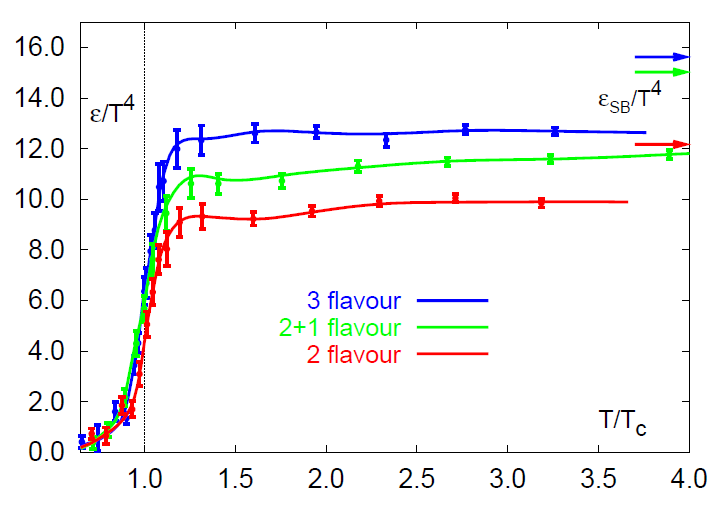
\includegraphics [width = 0.55\linewidth] {Intro/EnergyDensity_QCD.png}
		\caption{Результаты решеточной КХД [1] для плотности энергии / T4 как функции температуры, масштабированной критической температурой Tc. Обратите внимание на стрелки справа, указывающие значения предела Стефана-Больцмана.}
		\label{img:EnergyDensityQCD}  
	\end{figure}
\end{comment}

Схематическое изображение фазовой диаграммы ядерной материи в приближении нулевых масс верхнего и нижнего кварков ($m_{u,d} = 0$) и бесконечной массы странного кварка ($m_s = \infty$) представлено на рис. \ref{img:PhaseDiagram}.
%/* Следующий абзац из диплома Ильи */
В области низких температур ($T\approx 0$ МэВ) и барионных плотностей $\mu\approx 900$ МэВ вещество находится в состоянии адронного газа, при котором кварки находятся в состоянии конфаймента.  При при увеличении темепратуры и/или барионной плотности вещество переходит в состояние КГП, в котором кварки и глюоны находятся в состоянии асимптотической свободы [8]. Теоретические модели позволяют получить оценки границ такого перехода. В области низких температур (ниже критической точки) предсказывается фазовый переход первого рода в то время, как в области высоких температур – кроссовер. При условии относительно низких значений температур и достаточно высоких значений барионного химического потенциала вещество переходит в состояние цветовой сверхпроводимости.

% Считается, что при достаточно больших значениях барионного химического потенциала $\mu$ наблюдается фазовый переход первого рода между адронной материей и кварк-глюонной плазмой (КГП), а также трикритическая точка, ниже которой фазовый переход становится переходом второго рода.
Ненулевые значения масс легких кварков резко меняют картину: фазовый переход второго рода, обозначенный пунктирной линией на рис. \ref{img:PhaseDiagram}, становится плавным кроссовером, а трикритическая точка соответственно становится критической точкой, обозначающей конец перехода первого рода, обнаруженный при более высоких значениях $\mu$.

Переход из КГП в состояние адронного газа называют адронизацией кварк глюонной плазмы. Основными моделями адронизации КГП являются модель рекомбинации и модель фрагментации струн.

\begin{figure}[] 
	\center
	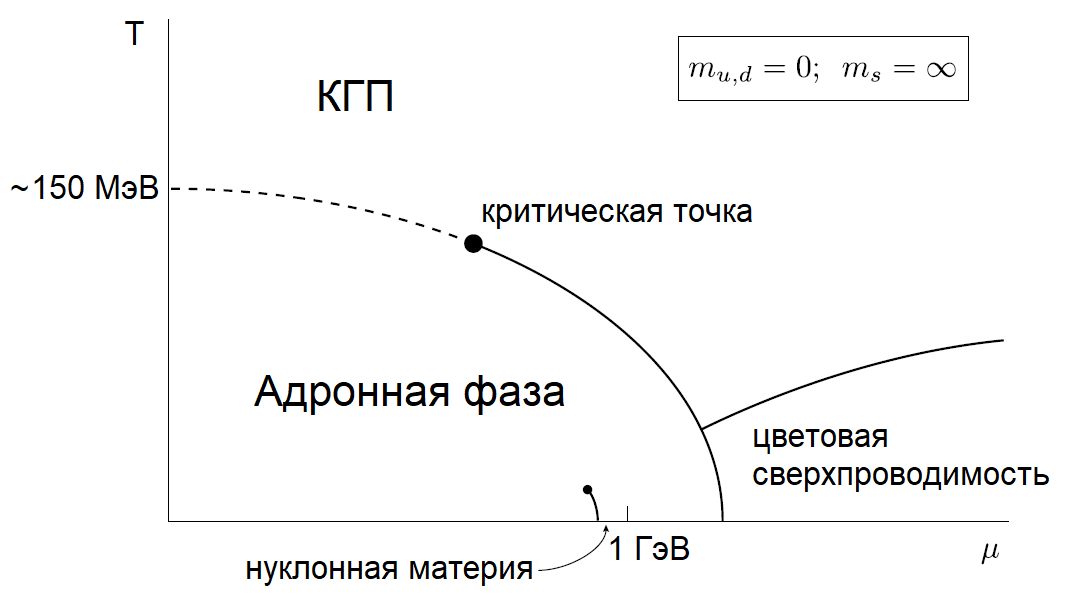
\includegraphics [width = 0.7\linewidth] {Intro/PhaseDiagram.png}
	\caption{Теоретическая фазовая диаграмма ядерной материи для двух безмассовых кварков в зависимости от температуры T и барионного химического потенциала}
	\label{img:PhaseDiagram}  
\end{figure}


Температура перехода соответствует плотности энергии $\epsilon = 1$ ГэВ/фм$^3$, что почти на порядок превышает плотность ядерного вещества $\epsilon_0 = 0.15$ ГэВ/фм$^3$[1407.5003]. Температуры и давления, необходимые для образования кварк-глюонной материи, достигаются в столкновениях тяжелых релятивистских ионоов.

Исследованию КГП в релятивистских столкновениях посвящены такие эксперименты, как PHENIX и STAR (BNL), ALICE(CERN), CBM(JSI), MPD(NICA) и другие.

Горячая, плотная материя, образующаяся в релятивистских столкновениях, проходит этапы пространственно-временной эволюции, показанные на рис  \ref{img:CollisionEvolution}.
Этапу формирования КГП предшествует предравновесная фаза. В момент времени $\tau_0$ ядерная материя переходит в состояние КГП. По мере расширения, КГП остывает и при достижении критической температуры $T_c$ происходит процесс адронизации - фазовый переход в нейтральную по цвету адронную материю. Кварки и глюоны объединяются в нейтральные по цвету объекты. Некоторое время ($\sim 4$ Фм/c) ядерная материя находится в смешанной фазе, состоящей из кварков и адронов. После завершения процесса адронизации наступает химическое равновесие и система полностью переходит в состояние адронного газа. После фазы адронного каскада наступает кинематическое равновесие, в котором не меняются импульсы частицы.
Адроны, образованные в результате столкновений тяжелы ионов, несут информацию о динамике столкновения и эволюции системы сталкивающихся ионов. Распределение по поперечному импульсу и выходы этих адронов являются наблюдаемыми, по которым можно судить о характеристиках ядерной материи, образованной в результате столкновения.

%Горячая и плотная материя, образующаяся в релятивистских столкновениях тяжелых ионов, может развиваться по следующему сценарию: предравновесие, тепловое (или химическое) равновесие партонов, возможное образование КГП или смешанного состояния КГП-адронный газ, газ горячих взаимодействующих адронов и, наконец, состояние замораживания, когда образовавшиеся адроны уже не сильно взаимодействуют друг с другом. На рис. \ref{img:CollisionEvolution} показана пространственно-временная эволюция среды, возникающей при столкновениях тяжелых ионов. Поскольку рожденные адроны несут информацию о динамике столкновений и всей пространственно-временной эволюции системы от начальной до конечной стадии столкновений, точная мера распределения поперечного импульса (pT) и выхода идентифицированных адронов в зависимости от геометрии столкновения необходима для пониманиядинамики столкновений и свойств созданной материи.


\begin{figure}[] 
	\center
	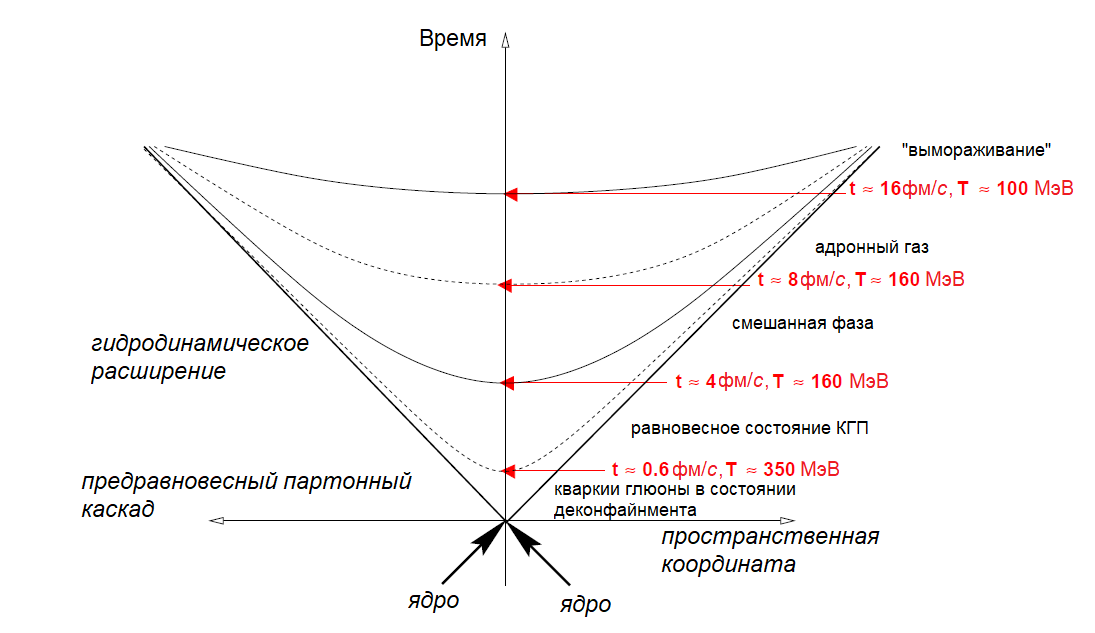
\includegraphics [width = 0.9\linewidth] {Intro/CollisionEvolution.png}
	\caption{Пространственно-временная картина ядерно-ядерного столкновения.}
	\label{img:CollisionEvolution}  
\end{figure}




\subsection{Процесс адронизации в столкновениях релятивистских тяжжелых ионов} \label{subsec:ch1/sec1_1}
Описание процесса адронизации представляет собой чрезвычайно сложную задачу, поскольку связанные адронные состояния непертурбативны в рамках КХД.
%В связи с этим особую важность имеют экспериментальные измерения рождения адронов в релятивистских столкновениях.
В настоящее время, для описания процессов адронизации преимущественно используется две модели: модель фрагментации и модель рекомбинации. 

%/* Fragmentation and Hadronization */
%Адронизация — это дальнодействующий процесс, включающий лишь небольшие передачи импульса. Следовательно, потоки энергии-импульса и квантовых чисел аромата на адронном уровне должны следовать потокам на партонном уровне. Результаты по инклюзивным спектрам и кратностям подтверждают эту гипотезу. Универсальный низкомасштабный $\alpha_s$ [19, 20, 21]. Теория возмущений хорошо работает вплоть до малых масштабов, $Q \sim 1$ ГэВ. Поэтому предположим, что $\alpha_s(Q^2)$ можно определить непертурбативно для всех $Q$, и использовать его при вычислении графов Фейнмана. Этот подход дает хорошее описание спектров тяжелых кварков и форм событий.
%Приведенные выше общие идеи не пытаются описать механизм образования адронов. Для этого мы пока должны прибегать к моделям. Основными современными моделями являются кластерная и струнная адронизация (рис. 2). Мы кратко опишем версии, используемые в генераторах событий HERWIG и JETSET соответственно.


\begin{comment}
	\textbf{Кластерная модель} [22]-[26]. Модель начинается с непертурбативного расщепления глюонов g → qq после партонного потока. Комбинации цвет-синглет qq имеют меньшие массы и универсальный спектр из-за свойства предконфайнмента [27, 28] ливня (рис. 3 [29]). Предполагается, что эти синглетно-цветовые комбинации образуют кластеры, которые в большинстве случаев подвергаются простому изотропному распаду на пары адронов, выбранные в соответствии с плотностью состояний с соответствующими квантовыми числами [23]. Эта модель имеет мало параметров и естественный механизм генерации поперечных импульсов и подавления рождения тяжелых частиц при адронизации. Однако у него есть проблемы с распадом очень массивных кластеров и с адекватным подавлением рождения барионов и тяжелых кварков.
	
	\textbf{Струнная модель} Эта модель основана на динамике релятивистской струны, представляющей собой цветовой поток, натянутый между исходными $q\bar{q}$. Струна создает линейный потенциал удержания и закон площадей для матричных элементов:
	$$|M(q\bar{q} \rightarrow h_1 ... h_n)|^2 \sim e^{-b A}$$
	где $A$ — заметаемая область пространства-времени (рис. 4). Струна распадается на адроны за счет образования пары $q\bar{q}$ в ее интенсивном цветовом поле. Глюоны, образующиеся в потоке партонов, вызывают «перегибы» на струне. Модель имеет дополнительные параметры для распределения поперечного импульса и подавления тяжелых частиц. У нее есть некоторые проблемы с описанием рождения барионов, но меньше, чем у кластерной модели.
	
	\textbf{Модель UCLA} [35]-[37] представляет собой вариант струнной модели JETSET, в которой приведенный выше закон площадей для матричных элементов рассматривается более серьезно и используется для определения относительных скоростей образования различных видов адронов. Это приводит к подавлению тяжелых частиц без дополнительных параметров, причем квадрат массы адрона пропорционален его площади в пространстве-времени. В настоящее время модель по-прежнему использует дополнительные параметры для $p_T$-спектров и снова имеет некоторые проблемы с описанием образования барионов.
\end{comment}
\subsubsection{Модель фрагментации} \label{sssec:ch1/sec1_2}

%/* Lund fragmentation */
Фрагментационные модели основаны на принципе конфайнмента и преимущественно применяются для описания процесса адронизации жестко рассеянного партона в элементарных столкновениях. 
%Потенциал сильного взаимодействия рамках КХД имеет следующий вид:
%
%где $\alpha_s \approx 1$ - константа сильного взаимодействия, а коэффициент $\kappa ~ 1$ ГэВ/c. Наличие линейного члена было впервые установлено с помощью адронной спектроскопии, а позже подтверждено расчетами КХД на решетке. На больших расстояниях ($r > 1$ фм) доминирует линейный член. В модели фрагментации только этот член используется для описания распада массивной qq-системы на несколько менее массовых. Тогда полное цветовое поле можно аппроксимировать одномерной струной, натянутой прямо между q и q, рис. 1. Эту струну можно рассматривать как параметризующую центр цилиндрической области одинаковой ширины по всей ее длине, так что продольные и поперечные степени свободы почти полностью развязаны.

Конфайнмент принято рассматривать [https://arxiv.org/pdf/1808.04619.pdf] как проявление линейного члена в потенциале сильного взаимодействия между кварком и антикварком ($q$, $\bar{q}$) в общем цветовом синглетном состоянии:
$$ V_{QCD}(r) \approx -\frac{4}{3} \frac{\alpha_s}{r} +\kappa \cdot r$$
где $r$ — расстояние между кварком и антикварком, $\alpha_{s}$ — константа сильного взаимодействия, $\kappa \approx 1$ ГэВ/фм.
Наличие линейного члена было впервые обнаружено с помощью адронной спектроскопии, а позже подтверждено расчетами КХД на решетке. 

Цветовое поле, возникающее при сильном взаимодействии двух цветовых зарядов ($q$, $\bar{q}$), можно представить в виде одномерной струны, натянутой между $q$ и $\bar{q}$, рис. \ref{img:Fragmentation}. 
При увеличении расстояния между $q$ и $\bar{q}$ струна растягивается, а величина потенциала $V_{QCD}(r)$ растет. Когда величина $V_{QCD}(r)$ превышает порог рождения кварк-антикварковой пары, происходит разрыв струны с дальнейшим формированием адронов.  
%Растяжение струны продолжается до тех пор, когда энергетичски более выгодным появление новой кварк-антикварковой пары, а не удлинение трубки
%При увеличении расстояния между двумя цветовыми зарядами, квакром и антикварком, вклад линейного члена $V_{QCD}$ растет. В какой-то момент становится энергетически выгодным появление новой кварк-антикварковой пары, а не удлинение трубки. В результате этого, когда кварки образуются в ускорителях частиц, вместо того, чтобы видеть отдельные кварки в детекторах, ученые видят "струи" из множества нейтральных по цвету частиц (мезонов и барионов), сгруппированных вместе. Этот процесс называется адронизацией, фрагментацией или разрывом струны.

\begin{figure}[] 
	\center
	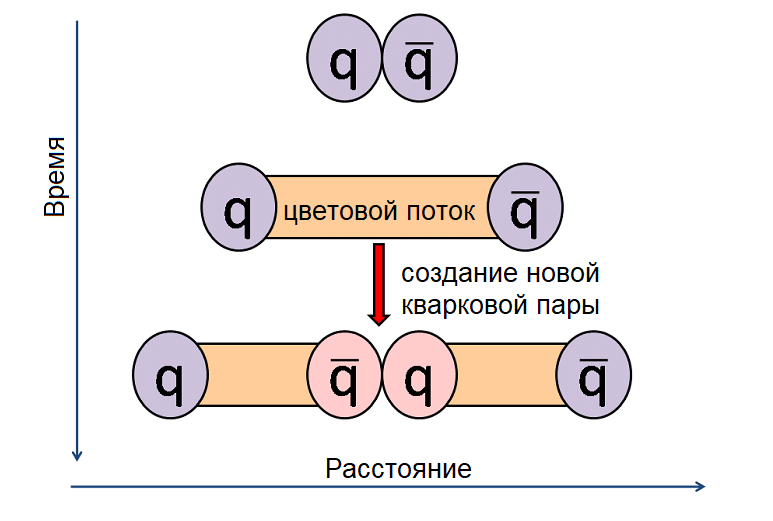
\includegraphics [width = 0.6\linewidth] {Intro/fragmentation model color}
	\caption{Формирование адронов согласно модели фрагментации.}
	\label{img:Fragmentation}  
\end{figure}


%Таким образом, модель фрагментации основана на нескольких общих предположениях: (i) частицы в конечном состоянии возникают в результате разрыва силового поля, похожего на струну, натянутого между цветовыми зарядами, (ii) существует причинность и лоренц-инвариантность и (iii) производство частицы могут быть описаны в терминах стохастического процесса, который подчиняется предположению о насыщении.

%Другой моделью адронизации является модель фрагментации, согласно которой адроны образуются из партонных струй. Согласно рекомбинационной модели, адроны образуются в результате рекомбинации партонов, близких друг к другу в фазовом пространстве. Фрагментация и рекомбинация являются конкурирующими механизмами, но рекомбинация естественным образом увеличивает соотношение барион/мезон при промежуточных $p_T$, поэтому считается, что фрагментация преобладает при высоких значениях $p_T$, а рекомбинация — при средних значениях $p_T$.
%Полагают, что при энергии 200 ГэВ в области поперечных импульсов $1.5$  ГэВ/c $\leq p_T \leq 3$ ГэВ/c процессы рекомбинации являются доминирующими в процессе адронизации КГП, а при более высоких поперечных импульсах ($p_T\geq 6$  ГэВ/c)  доминирующими являются процессы фрагментации. В области поперечных импульсов $3$  ГэВ/c $\leq p_T \leq 6$ ГэВ/c Модель рекомбинации и модель фрагментации являются конкурирующими.

\subsubsection{Модель рекомбинации} \label{sssec:ch1/sec1_3}
%/* Coalescence models for hadron Formation */
%Процесс адронизации из КГП может сильно отличает достижении термализации и образование большого количества партонов достигается термализация и не образуется масса партонов. В этом обзоре мы обсуждаем модель адронизации КГП путем слияния или рекомбинации кварков и глюонов. Обсуждаемые здесь модели успешно описывают многие существенные особенности образования адронов в столкновениях тяжелых ионов.
Согласно модели рекомбинации (коалесценции), адронизация КГП происходит в результате объединения кварков, находящихся в фазовом пространстве $(x, p)$ на расстоянии меньше радиуса рекомбинации $(\Delta_x, \Delta_p)$. Величины $\Delta_x, \Delta_p$, связанные соотношением неопределенностей $\Delta_p \cdot \Delta_x \approx 1$, являются параметрами рекомбинационной модели и определеяется исходя из соответствия экспериментальным данным.


\begin{comment}
	Количество мезонов, имеющих определенный импульс P может быть вычислено согласно следующей формуле
	$$\frac{dN_M}{d^3 P}=\sum_{a,b}\int \frac{d^3 R}{2\pi^3} \frac{d^3 q d^3 r}{2\pi^3}  W_{ab}(R-\frac{r}{2},\frac{P}{2}-q;R+\frac{r}{2},\frac{P}{2}+q) \Phi_M (r,q) $$
	Где индекс $M$ обозначает мезон, а индексы $a$ и $b$ обозначают коалесцирующие валентные кварки. $W_{ab}$ и $\Phi_M$ – функции Вигнера для партонов и мезона соответственно, $P$ и $R$ – импульс и координата мезона, $q$ и $r$ – доли импульса, которые несут кварки, и координаты кварков. Суммирование производится по всем возможным комбинациям 
\end{comment}

Количество адронов $N_n$, содержащих $n$ кварков/акнтикарков, имеющих координаты $x_i$ и импульсы $p_i$  может быть вычислено согласно формуле:
$$ N_n=g\int \prod_{i=1}^n p_i d\sigma_i  \frac{d^3 p_i}{(2\pi)^3 E_i }  f_{q,i} (x_i,p_i ) f_n(x_1,…,x_n;p_1,…,p_n ) $$
$g$-спин-цветовой статистический множитель.
Например, $g_\pi=g_K=1/36$, $g_p~=~g_{\bar{p}}~=~1/108$, $g_\rho~=~g_{K^*}~=~1/12$.

$f_q (x,p)$- функция распределения кварков 
$\int p\cdot d\sigma \frac{d^3 p}{(2\pi)^3 E} f_q(x,p)=N$

Функции вероятности образования мезона ($f_M$) и бариона ($f_B$) путем рекомбинации могут быть найдены следующим образом:
%$$f_M (x_1,x_2;p_1,p_2 )= exp{\frac{(x_1-x_2 )^2}{2\Delta_{x^2}}} \cdot exp{\frac{(p_1-p_2 )^2-(m_1-m_2 )^2}{2\Delta_{p^2} }}$$
$$f_M (x_1,x_2;p_1,p_2 )=\frac{9 \pi}{2\Delta_{x}^3 \Delta_{p}^3} \Theta \left( \Delta_{x}^2 - (x_1 - x_2)^2  \right) \times$$
$$ \Theta \left( \Delta_{p}^2 - (p_1 - p_2)^2  + \frac{1}{4}(m_1 - m_2)^2 \right) $$


$$f_B(x_1, x_2, x_3; p_1, p_2, p_3) = \frac{9 \pi}{2\Delta_{x}^3 \Delta_{p}^3} 
\Theta \left( \Delta_{x}^2 - \frac{1}{2} (x_1 - x_2)^2\right) \times $$
$$\Theta \left( \Delta_{p}^2 - \frac{1}{2} (p_1 - p_2)^2\right) \frac{9 \pi}{2\Delta_{x}^3 \Delta_{p}^3}\times
\Theta \left( \Delta_{x}^2 - \frac{1}{6} (x_1 + x_2 - 2 x_3)^2\right) \times $$
$$\Theta \left( \Delta_{p}^2 - \frac{1}{6} \left[ (p_1 + p_2 - 2 p_3)^2 - (m_1 + m_2 -2 m_3)^2 \right] \right) $$
В приведенном выражении для $f_B$ использовано приближение, согласно которому радиусы рекомбинации пространства и импульса одинаковы для трех кварков, формирующих барион. Нормировка функции $f_B$ аналогична нормировке функции вероятности коалесценции мезонов $f_M$, то есть, $(2\pi)^6$ после интегрирования по относительным координатам и моментам в нерелятивистском пределе. 

Заметим, что модель рекомбинации основана на предположении о доминировании валентных кварков, т.е. низшие фоковские состояния являются наиболее важными. 

Модель рекоминации реализована в пакете AMPT.

%/* Coalescence models for hadron Formation */
%Только модели коалесценции выдержали испытания, наложенные внушительным объемом данных, полученных после первоначального открытия барионного усиления. Они особенно привлекательны, потому что они, кажется, обеспечивают естественное объяснение масштабирования числа валентных кварков, которое наблюдалось в измерениях v2. Они также связывают адронные наблюдаемые с доадронной стадией взаимодействия кварков и глюонов. Таким образом, они касаются центральных вопросов программы физики тяжелых ионов: деконфайнмента и восстановления киральной симметрии.

\subsection{Признаки образования КГП} \label{subsec:ch1/sec1_1}
Существует ряд экспериментальных признаков, по которым можно судить о возможном образовании КГП в столкновении релятивистских тяжелых ионов. 

\textbf{Повышенный выход барионов}
В протон-протонных столкновениях в области поперечных импульсов $p_T \approx $3 ГэВ/с барионов рождается в 3 раза меньше, чем мезонов. Это связано с большими массами барионов и требованием ненулевого барионного числа для образования бариона.
Однако в 2002 году экспериментом PHENIX было обнаружено, что в центральных Au+Au столкновениях при энергиях 130 ГэВ, а в последствии и при 200 ГэВ, протоны(антипротоны) и $\pi^{\pm}$-мезоны рождаются примерно в равной пропорции (отношение выходов протонов к выходам $\pi$-мезонов ($p/\pi$) достигает значения 0.8). С уменьшением центральности столкновений различие между значениями $p\pi$, измененными в p+p и Au+Au взаимодействиях уменьшается. Единственной моделью, способной объяснить данную аномалию, получившую название «барионная загадка», оказалась модель рекомбинации.

%Данный эффект был объяснен в рамках двух моделей: модели гидродинамики и модели кварковой коалесценции. В рамках модели гидродинамики [16,17], полагают локальное тепловое равновесие партонной/адронной материи в начальный момент времени, описывающее в последствии пространственное-временное изменение термализованной материи, путем решения уравнения сохранения энергии – импульса. Данная модель довольно успешной объясняет увеличение отношений выходов барионов к мезонам.

% Cronin peak paper
%На этой конференции было признано, что среда влияет на динамику адронизации. Первый намек [1] на то, что в столкновениях Au+Au на RHIC барионы образуются по-другому, был получен наблюдением того, что в центральных столкновениях вблизи $p_T \sim $2 ГэВ/c выходы протонов и антипротонов сравнимы с выходом пионов, вопреки ожиданиям, основанным на известных функциях фрагментации. Масштабирование выхода протонов и антипротонов по центральности [2] также с трудом укладывается в мягкое+жесткое описание адронных спектров. Большое количество идентифицированных адронных измерений, доступных в настоящее время [2-6], делает возможным детальное изучение массовых эффектов по сравнению с барионными/мезонными эффектами. Стало очевидным, что наблюдаемые явления специфичны для столкновений ядро-ядро и могут быть связаны с числом кварков в адроне. Разрешение "барионной аномалии" является основной темой данного выступления. Презентация ориентировано на эксперимент. После краткого обзора мягкой физики (раздел 2) и жесткой физики (раздел 3), я попытаюсь провести систематический обзор промежуточных результатов по $p_T$ в столкновениях Au+Au и d+Au. (Раздел 4). Теоретически мало известно о вкусовой зависимости эффекта Кронина и о особенности адронизации как в присутствии, так и в отсутствии QGP среды. Есть надежда, что что экспериментальные исследования, подобные этому, помогут направить теорию дальше описания "только пионов только". В данной работе основное внимание уделяется данным RHIC по средней скорости, а обсуждение в основном сосредоточено на идентифицированных адронных спектрах.
\textbf{Повышенный выход странности}
Одним из признаков образования КГП считается повышенный выход частиц, содержащих странный кварк. При рождении кварк – антикварковой пары в релятивистских протон-протонных столкновениях, выходы адронов, содержащих тяжелые кварки, подавляются в связи с их большой массой. В столкновениях тяжелых релятивистских ионов, при условии формирования КГП, выход странных кварков увеличивается за счет вклада глюн-глюонного рассеяния. В связи с этим повышенный выход странности может быть одним из признаков образования КГП. 
%Механизм образования странных кварков представлен на рис. \ref{img:StrangenessEnhancement}.

%Наиболее часто предлагаемые сигнатуры для возможного наблюдения КГП - это увеличение странности и появление антибарионов. В образовании пары $\bar{q}q$ при столкновении нуклонов и нуклонов высоких энергий тяжелые ароматы подавляются из-за их массы. Выход $\bar{s}s$  составляет около 0,1 $\gg$ 0,2 по сравнению с выходами $\bar{u}u$  или $\bar{d}d$. Эта ситуация может измениться при столкновениях тяжелых ионов. Если адронная материя деконфайнментируется во время столкновения тяжелых ионов, то образование u- и d-кварков будет подавлено блокировкой Паули. Следовательно, усиление странности может быть одним из сигналов КГП.
\begin{comment}
	\begin{figure}[] 
		\center
		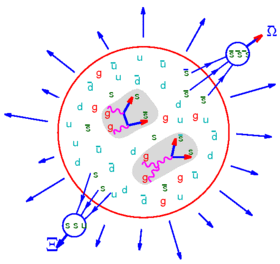
\includegraphics [width = 0.5\linewidth] {Intro/Strangeness_enhancement.png}
		\caption{Механизм образования странных кварков, основанный на модели термальной КХД.}
		\label{img:StrangenessEnhancement}  
	\end{figure}
\end{comment}
\begin{comment}
	\textbf{Динамика столкновения и уравнение состояния}
	Ожидается, что изучение коллективного движения образовавшихся адронов в конечном состоянии даст информацию о динамике столкновений тяжелых ионов. С гидродинамической точки зрения на столкновения,
	коллективное движение определяется градиентом давления сжатой ядерной материи на ранней стадии столкновения. В случае фазового перехода от порядковой ядерной к кварк-глюонной плазме ожидается соответствующее смягчение уравнения состояния за счет увеличения числа степеней свободы [4]. Таким образом, наблюдение за коллективным движением крайне важно для подтверждения гидродинамического описания динамики. Если фазовый переход первого рода, то уравнение состояния будет наиболее «мягким» при критической температуре Tc. Ожидается, что такое смягчение повлияет на динамическую эволюцию системы, поскольку внутреннее давление падает при Tc. Таким образом, наблюдение за функцией возбуждения поперечного коллективного потока может служить зондом для формирования КГП; падение функции возбуждения коллективного потока свидетельствует о пороговой энергии образования КГП.
\end{comment}

\textbf{Потери энергии партонами}
Спектры адронов с большим поперечным импульсом ($p_T$), образующихся в результате фрагментации сильно рассеянных партонов, потенциально могут служить прямым исследованием свойств начального состояния. В столкновении тяжелых релятивистских ионов фаза жестких рассеяний предшествует образованию КГП. Таким образом, высокоэнергетичные партоны, участвовавшие в жестких рассеяниях, впоследствии испытывают взаимодействие с кварк–глюонной средой, теряя энергию. Предположительно, партоны теряют энергию [15] в горячей и плотной ядерной материи в следствии глюонного тормозного излучения, эффективно гасящего образованные струи. Одним из следствий данного эффекта является уменьшение выхода адронов высокой энергии ($p_T > $5 ГэВ/с). 

% Cronin peak paper
%Выше $T \sim $2 ГэВ/c все большее значение приобретают процессы жесткого рассеяния. Они обеспечивают чувствительный инструмент для исследования образующейся среды. После жесткого рассеяния цветной объект (жестко рассеянный кварк или глюон) пересекает среду, образовавшуюся в результате столкновения, и сильно взаимодействует. В результате ожидается, что он потеряет энергию через индуцированное глюонное излучение. Это явление, известное как тушение струи, проявляется в виде подавления выхода адронов с высоким $p_T$ адронов, по сравнению с производством в pp-столкновениях, масштабируемым ядерной толщиной функцией $T_{AB}$, которая учитывает ядерную геометрию. Подавление измеряется в терминах фактор ядерной модификации $R_{AA} = \sigma^{AA}/T_{AB} \sigma ^{pp}$. Адронные спектры от pp-столкновений служат в качестве эталона, свободного от ядерных эффектов, и будут обсуждаться здесь в этом контексте. Важно также важно различать ядерные эффекты в начальном состоянии (холодная ядерная материя) и в конечного состояния (предположительно QGP). В RHIC столкновения d+Au при той же энергии центра масс, что и столкновения Au+Au служат этой цели. Эффект Кронина, который обычно приписывается начальному множественному рассеянию в начальном состоянии, изучается подробно.

%Другой возможный способ исследования кварк-глюонной плазмы — потеря энергии быстрым партоном (кварком или глюоном). Механизмы аналогичны тем, которые ответственны за потерю электромагнитной энергии быстрой заряженной частицей в веществе, т. е. потеря энергии может происходить либо на возбуждение проникшей среды, либо на излучение. Быстрый партон может производить адрон с высоким pT, измерение образования адронов с высоким pT является хорошим зондом для изучения потери энергии партонов. Более подробная информация описана в Разделе 1.3.

\textbf{Коллективные потоки}
В периферийных столкновениях зона перекрытия ядер имеет миндалевидную форму (рис. 2.4.). В следствии анизотропии области перекрытия, в сгустке материи образуются градиенты давления. В плоскости реакции давление стремится к максимально возможному. В результате расширения и остывания образовавшегося файербола, в следствии анизотропии давления, азимутальное импульсное распределение частиц также становится анизотропным. Количественный анализ азимутального распределения частиц в анизотропии определяется посредством Фурье разложения одночастичного распределения частиц по азимутальному углу $\phi$[12]:
$$ E \frac{d^3N}{dp^3} = \frac{1}{2\pi} \frac{d^2N}{p_T dp_T dy} 
(1+\sum_{n=1}^{N} 2v_n cos(n(\phi - \psi)))$$
где $E$ - энергия частицы, 
$p_T$ - поперечный импульс,
$y$ - быстрота частицы, 
$\phi$ - азимутальный угол частиы, 
$\psi$ - угол плоскости реакции, 
$v_n$ - коллективный поток порядка $n$. 
Величина эллиптического потока позволяет получить информацию о значениях градиентов давления при гидродинамическом расширении, эффективных степенях свободы и степени термализации на ранних этапах. Зависимость эллиптического потока от размера системы, поперечного импульса или массы, имеют важнейшее значение для понимания свойств материи, образующейся во время столкновений. 
В центральных столкновениях эллиптический поток меньше, по сравнению с перифирийными столкновениями. Это связано с тем, что в центральных столкновениях область перекрытия ядер более округлая.

\textbf{Подавление тяжелых кваркониев}
Механизм подавления следует из ожидаемой дебаевской экранировки в КГП, уменьшающей диапазон потенциалов между $c\bar{c}$  парами [2, 3]. Если радиус мезона больше дебаевского радиуса, определяемого соотношением температуры и плотности плазмы, мезон распадается.

\begin{comment}
	Предполагается, что $J/\Psi$-мезон, состоящий из $c\bar{c}$-кварков, подходит для обнаружения эффекта экранирования Дебая по следующим причинам; 1) поскольку  $J/\Psi$-мезон измеряется в лептонном распаде, продукты распада не сильно взаимодействуют с другими адронами, поэтому ожидается проникающий зонд для ранней стадии столкновений, 2)  $J/\Psi$-мезон рождается на очень ранней стадии столкновение, 3) адронное взаимодействие  $J/\Psi$-мезон ожидается не слишком высоким (sYN $\gg$ 6 мб), таким образом, оно имеет информацию об условии начального состояния столкновений.
\end{comment}

\section{Рождение частиц в столкновениях релятивистских ионов}

Гидродинамическая модель, предложенная в 1950-х годах [13], считается одной из наиболее эффективных моделей для описания множественного рождения частиц.
Согласно гидродинамической модели в столкновениях релятивистских тяжелых ионов   на стадии образования КГП результате сильного взаимодействия устанавливается статистическое равновесие. Образовавшаяся КГП рассматривается как релятивистская жидкость, обладающая коллективным потоком.

Горячая и плотная материя, образовавшаяся в результате столкновения, увеличивается в размерах за счет образования множества частиц.
Таким образом, система достигает состояния достаточно высокой степени теплового и химического равновесия с достаточно большим числом частиц внутри, что позволяет применить статистические тепловые модели.
Затем фаза КГП сменяется смешанной фазой КГП + HRG (hadron resonanse gas)[Particle ratios in non ideal HRG], предполагающей фазовый переход первого порядка. После завершения процесса фазового перехода первого порядка частицы (т.е. адроны) в фазе адронного газа продолжают взаимодействовать. Адронные столкновения могут привести к высокой степени теплового и химического равновесия для различных видов адронов в фазе HRG. Система HRG продолжает расширяться и охлаждаться. Когда средние свободные пути этих частиц становятся сравнимыми с общим размером системы происходит кинетическое вымораживание.

Согласно термодинамическим моделям, количество частиц в КГП не фиксировано и описывается в рамках статистической физики большим каноническим ансамблем для каждого типа частиц:
$$\Omega_{GC} = -kT ln(Z)$$
где $k$ – постоянная Больцмана, 
$T$ – температура, 
$Z$- статистическая сумма, вид которой зависит от того, подчиняется ли частица статистике Бозе-Эйнштейна или статистике Ферми-Дирака.

Множественность рождения адрона типа $h$ описывается формулой (1.2):
$$ N_h = V\cdot n_h = \frac{V g_h}{(2 \pi \hbar)^2} \int f_h(p)d^3p$$
где $n_h$ – число степеней свободы,
$g_h=2J_h+1$ – фактор спинового вырождения,
$f_h(p)$- функция распределения импульса !!!.

Адронный химический потенциал – то, что отличает адроны друг от друга. Величины, которые сохраняются при взаимодействии частиц в адронном газе – барионное число, заряд и странность. Тогда химический потенциал представляет собой линейную комбинацию трех потенциалов:
$$\mu_h=h_B B_h + \mu_Q Q_h + \mu_S S_h$$
где $B_h$ – барионное число адрона $h$, 
$Q_h$- зарядовое число адрона $h$, 
$S$ -  странность адрона $h$.
Данная формула может быть расширена добавлением потоенциалов для C (charm) и B (bottomness) кварков.

%Гидродинамическая модель объясняет повышенный выход $p/\pi$. Однако, данная модель не предсказывает (или предсказывает, но очень слабую) зависимость данной величины от центральности столкновения. [10]

%Рождение частиц в столкновениях релятивистских тяжелых ионов принято описывать с помощью гидродинамических моделей. Согласно гидродинамическим моделям, процесс рождения адронов объясняется наличием расширяющегося поля поперечных скоростей при постоянной температуре термализованной системы.
%Отношения инвариантных спектров частиц чувствительны к химическим свойствам системы и механизму образования частиц. 

В случае чисто теплового движения все частицы (независимо от их массы) двигаются с одной и той же средней кинетической энергией, определяемой температурой, т.е.
$$\langle E_{kin} \rangle \sim T_{thermal}$$
С другой стороны, в случае абсолютного коллективного движения все частицы двигаются с одинаковой поперечной скоростью $\beta{T}$ и следовательно, их кинетическая энергиях пропорциональна массе:
$$\langle E_{collective} \rangle \sim \frac{m_0 u_T ^2}{2} $$
В предположении полного независимости теплового и коллективного движения частицы полная кинетическая энергия будет равна:
$$ \langle E_{kin} \rangle = \langle E_{thermal} \rangle + \langle E_{collective} \rangle = T_{thermal}+\frac{m_0 \langle u_T ^2 \rangle }{2}$$
где $ \langle u_T ^2 \rangle$ - средняя коллективная поперечная скорость для частиц всех типов. 



\section{Столкновения легких систем}

К малым системам столкновений относятся такие системы как p+Al, p+Au, d+Au, He+Au. Долгое время считалось, что в малых системах столкновений не достигаются значения температур и давлений, необходимые для образования КГП. В связи с этим, рождение частиц в малых системах столкновений изучалось преимущественно с целью исследования эффектов холодной ядерной материи, таких как эффект Кронина, многократное рассеяние партонов, модификации начальных функций распределения ядерных партонов (PDF) и т.д.

%Экспериментальное изучение столкновений тяжелых ядер при релятивистских энергиях позволило установить свойства кварк-глюонной плазмы (КГП), состояния горячей, плотной ядерной материи, в которой кварки и глюоны не связаны в адроны [14]. В этом состоянии материя ведет себя как почти невязкая жидкость [5], которая эффективно переводит начальные пространственные анизотропии в коррелированные анизотропии импульса среди образовавшихся частиц, создавая общий паттерн скорости, известный как коллективный поток. В последние годы сравнимые анизотропии импульса были измерены в столкновениях малых систем протон-протон (p+p) и протон-ядро (p+A), несмотря на ожидания, что объем и время жизни образующейся среды будут слишком малы для формирования QGP. Здесь мы сообщаем о наблюдении эллиптических и треугольных потоков заряженных частиц, образующихся в столкновениях протон-золото (p+Au), дейтрон-золото (d+Au) и гелий-золото (3He+Au) при энергии нуклон-нуклонного центра масс $\sqrt{s_{NN}}$ = 200 ГэВ. Уникальное сочетание трех различных начальных геометрий и двух схем течения обеспечивает беспрецедентную дискриминацию моделей. Гидродинамические модели, включающие образование короткоживущей капли QGP, обеспечивают одновременное описание этих измерений.

\subsection{Эффекты холодной ядерной материи}
%J/Psi Phenix results
Эффекты CNM известны как любые изменения в процессах рождения частиц, не вызванные горячей и плотной средой, образующейся в столкновении [12]. 

%В сообществе до сих пор ведутся открытые дебаты о точном определении эффектов начального и нального состояния. В частности, существует некоторая неопределенность в вопросе о том, следует ли обозначать ядерное поглощение как initial-state effects" - эффекты CNM, включая ядерное поглощение, и final-state effects" - эффекты, обусловленные энергией, выделяющейся при столкновении. Ожидается, что эффекты начального и конечного состояния будут разными при энергиях RHIC и LHC, поэтому сравнение PHENIX с измерениями LHC особенно ценно. 
%В последние годы в сообществе физиков высоких энергий большое внимание уделяется экспериментам, которые указывают на плавный переход между "малыми" системами столкновений (протон-протон, pp и протон-ядро, pA [39]) и "большими" системами столкновений. (ядро-ядро, АА [39]). Эти результаты, полученные как на Большом адронном коллайдере (LHC), так и на релятивистском коллайдере тяжелых ионов (RHIC), особенно поразительны, поскольку некоторые из наблюдаемых традиционно рассматривались как сигнатуры создания партонной материи в состоянии деконфайнмента, близкой к термодинамическому равновесию - кварк-глюонной плазмы - в высокоэнергетических столкнове-ниях АА. Они включают азимутальные асимметрии коллективной природы, термически подобные спектры и повышенный выход барионов и странности при малом и промежуточном поперечном импульсе соответственно, подавление кваркония, единственным исключением является гашение струй. Эти сигнарту-ры успешно описываются с помощью расчетов в рамках модели гидродинамики почти невязкой жидкости. Это означает, что в столкновениях тяжелых ионов образуется сильно взаимодействующая, почти идеальная жидкость [40].
%Обнаружение таких же, как и при столкновениях тяжелых ионов, сигналов азимутальной анизотропии в различных малых системах столкновений (таких как p + Au, d + Au, He + Au [39]) радикально изменило взгляд на минимальные условия, необходимые для образования КГП. Считалось, что размер системы в таких столкновениях слишком мал, чтобы создать какое-либо значительное ко-личество горячей ядерной материи, время жизни которой, к тому же, будет очень коротким [41]. Следовательно, в малых системах столкновений описание коллективного поведения в рамках гидродинамического расширения КГП тре-бует дальнейшего изучения.
%С теоретической стороны увеличивает важность этих результатов тот факт, что вязкая релятивистская гидродинамика способна дать описание данных даже в столкновениях малых систем, когда не достигаются условия большой непро-зрачности и приближенной изотропии импульса. В этом случае такие эффекты начального состояния, называемые эффекта-ми холодной ядерной материи (cold nuclear matter CNM), должны быть в любом случае рассмотрены как с фундаментальной точки зрения [45]. 


\textbf{Эффект Кронина}
Экспериментальные доказательства эффектов холодного ядерного вещества были впервые обнаружены в конце 1970-х годов, когда было обнаружено, что отношение сечений рождения адронов в $p$+A и p+p столкновениях зависит от величины $p_T$ [7,8]. В области малых поперечных импульсов ($p_T < $2 ГэВ/c) наблюдалось подавление выходов адронов, в области средних поперечных импульсов (2-5 ГэВ/c) выходы адронов повышались, однако, данное повышение выходов адронов исчезает при больших $p_T$ ($p_T > 5$ ГэВ/с).
Данная зависимость сечения рождения адронов от величины $p_T$ была названа "эффектом Кронина". Исторически эффект Кронина приписывался жесткому рассеянию в начальном состоянии [9,10]. Недостатком такого подхода является невозможность  объяснить гораздо больший эффект для протонов по сравнению с пионами. Измерения инвариантных $p_T$ спектров адронов экспериментами PHENIX и STAR при энергиях коллайдера RHIC в начале 2000-х годов возобновили интерес к эффекту Кронина.  На сегодняшний день не существует полного количественного объяснения эффекта Кронина. Большинство моделей, описывающих эффект Кронина, основаны на жестком и мягком многократном рассеянии [11-15], однако существуют подходы,использующие глюонное насыщение или адронизацию путем рекомбинации кварков [17].

Рассмотрим подходы, основанные на многократном рассеянии.
В случае, когда функция распределения партонов $f_{b/A}(x_b, k_b^2, T)$ имеет нормированную гауссову форму, случайное упругое рассеяние вызывает дальнейшее $k_T$-расширение в ядре:

$$\left< k_{b,T}^2 \right>_{pA} = \left< k_{b,T}^2 \right>_{pp} + \left< \frac{2 \mu^2 L}{\lambda_{q,g}} \right> \xi $$
где $k_{b,T}$ - поперечная компонента партона в ядре-мишени, $\xi = ln(1+\delta p_T^2)$. Значения параметров определены с помощью экспериментальных данных и составляют $\delta = 0.14$ ГэВ$^2$, $\mu^2 = 0.12$ ГэВ$^2$ и $\lambda_g = 1$фм.

\textbf{Потеря энергии в начальном состоянии холодной ядерной материи}
Партоны наслетающего протона претерпевают многократное рассеяние в ядре перед жестким столкновением, вследствии чеготеряют энергию из-за индуцированного средой тормозного глюонного излучения. Этот эффект может быть рассчитан через сдвиг доли импульса в партоных функциях распределения протона-снаряда,
$$f_{q/p}(x_a) \rightarrow f_{q/p} \left( \frac{x_a}{1-\varepsilon_{eff}} \right)$$
где $x_a$ - доля импульса протона-снаряда [20]. Многократное излучение глюонов, $\Delta E = \sum_i \Delta E_i$, уменьшает влияние средней потери энергии, что реализуется через соотношение $\varepsilon_{eff}=0.7(\Delta E / E)$. Средняя потеря энергии зависит от передачи импульса при взаимодействии, $\mu$, между партоном и средой и длиной свободного пробега глюона, $\lambda_g$. 

\textbf{Эффекты изоспина}
Эффект изоспина оказывает влияние на наблюдаемые, чувствительные к аромату кварков, например, к рождению фотонов или инклюзивному рождению адронов и не оказывает существенного влияния на процессы, в которых преобладают глюоны в начальном состоянии, такие как струи и тяжелые ароматы. 

Для оценки величины эффекта изоспина используются партонные функции распределения нуклонов в ядре с атомной массой $А$ и зарядом $Z$:
$$f_{a/A}(x) = \frac{Z}{A}f_{a/p}(x)+\left(1-Z/A \right) f_{a/n}(x)$$
где $f_{a/p}(x)$ и $f_{a/n}(x)$ - партонные функции распределения протона и нейтрона соответственно. 

\textbf{Динамическое затенение}
Последовательное когерентное рассеяние партонов-участников приводит к затенению в высших порядках наблюдаемого сечения. Этот эффект может быть учтен путем изменения доли импульса партонных функций распределения ядра-мишени:
$$x_b \rightarrow x_b \left(1+C_d  \frac{\xi^2 (A^{1⁄3}-1)}{-\hat{t}} \right)$$
где $x_b$ - доля импульса партона в ядре-мишени. Здесь $\xi ^2$ = 0,12 ГэВ$^2$ – характерный масштаб энергии многократного рассеяния. 


Требуются обширные экспериментальные измерения, чтобы понять и количественно оценить все эти эффекты в адрон-ядерных столкновениях. С этой целью PHENIX проводит измерения столкновений легких систем.


\subsection{Поиски признаков образования КГП в легких системах}

В 2018 г экспериментом ФЕНИКС были измерены эллиптические и триангулярные потоки заряженных частиц в столкновениях  p+Au, d+Au, He+Au при энергии 200 ГэВ. Полученные результаты были описаны в рамках модели гидродинамики, предпологающей формирование КГП. С тех пор поиск эффектов КГП в малых системах столкновений является актуальной задачей фузики высоких энергий. В настоящее время, помимо коллективных потоков, в столкновениях легких систем обнаружены такие признаки образования КГП как повышенный выход барионов, Гашение струй $pi0$ PHENIX results и $J/\Psi$ в легких системах. 

\textbf{Эллиптические и триангулярные потоки в p/d/He+Au столкновениях.}
На рис. \ref{img:CollectivitySmallSysts} представлено сравнение значений эллиптических и триангулярных потоков vn($p_T$), измеренных экспериментом PHENIX в центральных (0-5\%) a)p+Au b) d+Au, c) He+Au столкновениях с теоретическими  предсказаниями моделей SONIC, iEBE-VISHNU и MSTV. Данные модели используют гидродинамический подход к описанию столкновений релятивистских тяжелых ионов. 

\begin{figure}[] 
 \centerfloat
	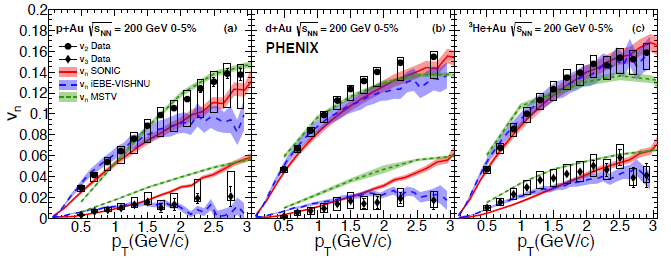
\includegraphics [width = 0.8\linewidth] {Intro/Collectivity_small_systs.png}
	\caption{Сравнение значений эллиптических и триангулярных потоков vn($p_T$), измеренных экспериментом PHENIX в центральных (0-5\%) a)p+Au b) d+Au, c) He+Au столкновениях с теоретическими  предсказаниями. Каждая точка представляет собой среднее значение по бинам pT шириной от 0.2 ГэВ/c до 0.5 ГэВ/c; черные кружки - v2, черные ромбы - v3. Сплошными красными (пунктирными синими) линиями представлены предсказания гидродинамических моделей sonic (iEBE-VISHNU). Сплошными зелеными кривыми представлены корреляционные постпрогнозы vn из MSTV по импульсу начального состояния.}
	\label{img:CollectivitySmallSysts}   
\end{figure}


\textbf{Заряженные адроны}
Экспериментом PHENIX были измерены факторы ядерной модификации заряженных адронов (рис. \ref{img:CH_RAA_dAu}) и отношения выходов $p/\pi$ в столкновениях d+Au (рис. \ref{img:p2pi_dAu}). 
Наблюдается повышенный выход протонов и антипротонов в центральных столкновениях d+Au, однако отношения выходов $p/\pi$ близки к значениям $p/\pi$, измеренным в p+p столкновениях, и не проявляют статистически значимой зависимости от центральности.
Полученные результаты могут быть интерпретированы как намек на образование КГП в столкновениях d+Au.
\begin{figure}[] 
	\centerfloat
	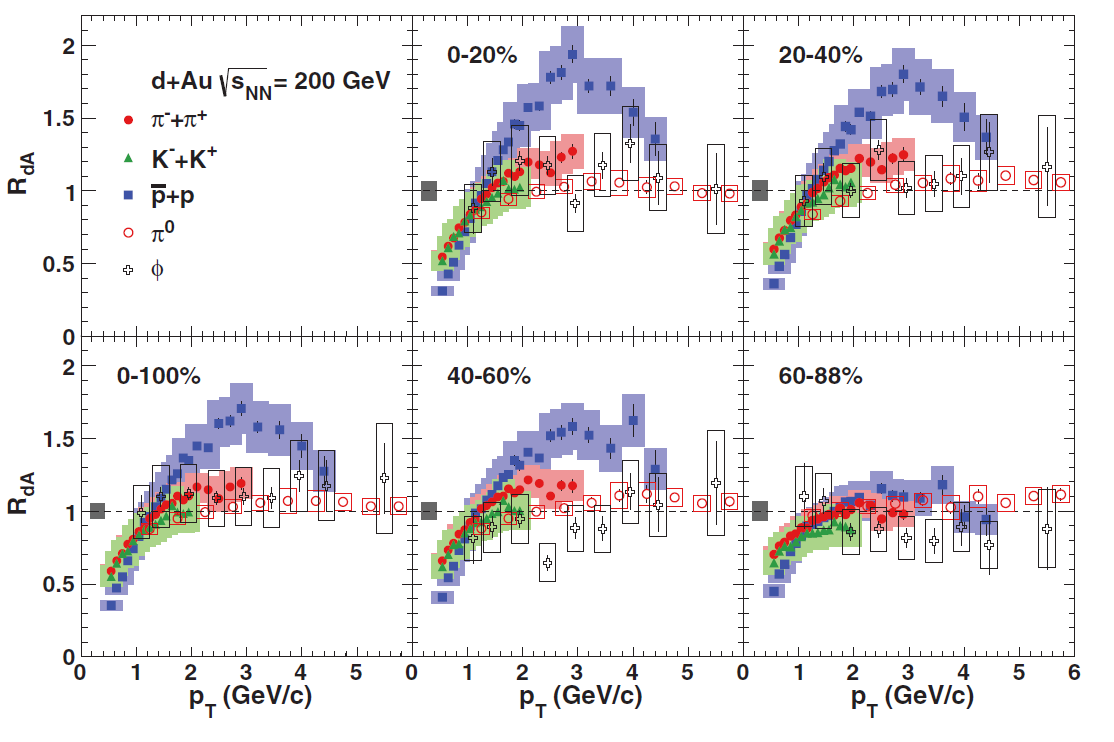
\includegraphics [width = 0.8\linewidth] {Intro/BaryonEnhancement_dAu.png}
	\caption{Факторы ядерной модификации заряженных адронов ($\pi^{+} + \pi^{-}$, $K^{+} + K^{-}$, $\bar{p}+p$, $\pi^0$, $\phi$), измеренные экспериментом PHENIX в столкновениях d+Au при энергии $\sqrt{s_{NN}}=$200 ГэВ.}
	\label{img:CH_RAA_dAu}   
\end{figure}

\begin{figure}[] 
	\centerfloat
	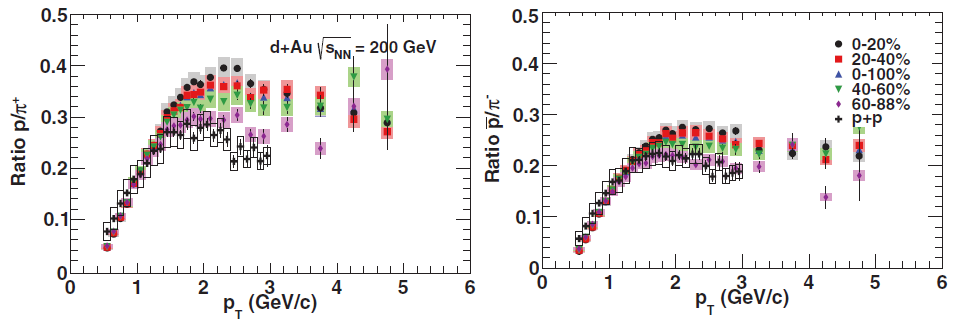
\includegraphics [width = 0.8\linewidth] {Intro/p2pi_dAu.png}
	\caption{Отношения выходов протонов к выходам $\pi^+$-мезонов ($p/\pi^{+}$) и выходов антипротонов к выходам $\pi^-$-мезонов ($\bar{p}/\pi^{-}$), измеренные экспериментом PHENIX в столкновениях d+Au при энергии $\sqrt{s_{NN}}=$200 ГэВ.}
	\label{img:p2pi_dAu}   
\end{figure}

\textbf{Гашение струй $pi0$ PHENIX results}
%pi0 in small systs PHENIX results
%Измерения распределений поперечного моментума ($p_T$) частиц, образующихся в адронных столкновениях, обычно используются для получения информации о взаимодействии. На Релятивистском коллайдере тяжелых ионов (RHIC) в Брукхейвенской национальной лаборатории (Brookhaven National Брукхейвенской национальной лаборатории, изучается фактор ядерной модификации RAA адронов, определяемого как отношение выхода адронов на бинарное нуклон-нуклонное столкновение в данной системе A + A к выход, измеренный в p + p столкновениях, привели к значительным открытиям. открытиям.
Обнаружение подавления нейтральных пионов и заряженных адронов [1,2] в области больших $p_T$ ($p_T > 5$ ГэВ/c) в столкновениях Au+Au по сравнению с p+p столкновениями при той же энергии, было одним из первых намеков на потерю энергии партонами в сильно связанной КГП. Отсутствие подавления высокоэнергетичных адронов в столкновениях d+Au [3,4], в которых образование КГП не ожидалось, было критически важным для установления потери энергии партонов в качестве причины наблюдаемого подавления в столкновениях Au+Au. Последующие систематические исследования подавления рождения высокоэнергетичных $\pi^0$ в столкновениях Au+Au при $\sqrt{s_{NN}}$ = 200 ГэВ позволили получить количественные ограничения на коэффициенты переноса среды [5,6].



\textbf{$J/\Psi$ в легких системах}

\begin{figure}[] 
	\centerfloat
	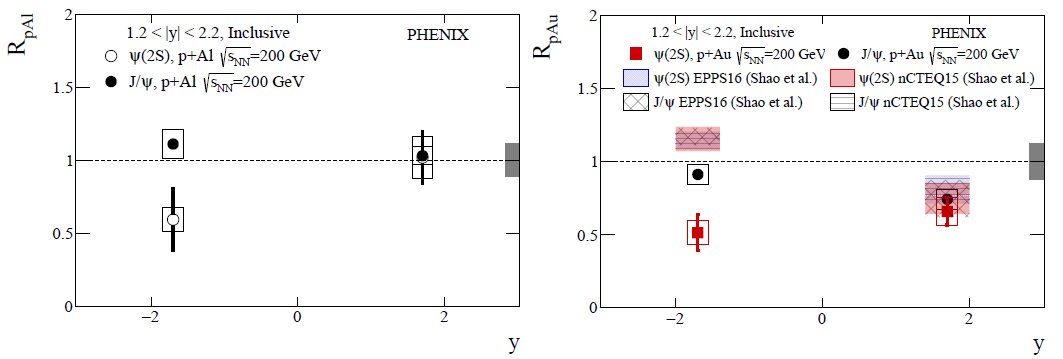
\includegraphics [width = 0.8\linewidth] {Intro/JPsi_SmallSysts}
	\caption{$J/\Psi$ в столкновениях p+Au и p+Al. }
	\label{img:CollisionEvolution}  
\end{figure}

на релятивистском коллайдере тяжелых ионов (RHIC) экспериментом PHENIX наблюдалось подавление состояния кваркония $\Psi(2S)$ в d+Au столкновениях при энергии $\sqrt{s_{NN}}=$200 ГэВ, что является возможным признаком эффектов нального состояния [8]. Подавление факторов ядерной модификации $\Psi(2S)$ позднее наблюдалось на Большом адронном коллайдере (БАК) коллаборациями ALICE и LHCb в столкновениях p+Pb [9, 10]. Результаты измерений $\Psi(2S)$ были опубликованы после анализа факторов ядерной модификации $J/\Psi$ в d+Au столкновениях, который показал, что за подавление выходов $J/\Psi$ в d+Au столкновениях по сравнению с p+p столкновениями ответственны эффекты холодной ядерной материи (CNM) [11].
При энергиях БАК аналогичные результаты по подавлению выходов $J/\Psi$ были опубликованы в p+Pb столкновениях [19, 20] и также в основном согласуются с эффектами CNM. В целом, $J/\Psi$ ядерная модификация в различных экспериментах согласуется с эффектами КНМ, в то время как подавление, наблюдаемое в $\Psi(2S)$ ядерной модификации, сильнее по отношению к $J/\Psi$ ядерной модификации, чем предсказывается эффектами КНМ. 



\section{Геометрия столкновений тяжелых ионов}
Cхема столкновения тяжелых ионов изображена на рис. \ref{img:CollisionGeometry}. Ось столкновения ядер сонаправлена оси z. %Плоскость, образованную прицельным параметром (b) и осью z, называют плоскостью реакции.  
Нуклоны, испытавшие хотя бы одно неупругое столкновение, называют нуклонами-участниками. Нуклоны, которые не испытали столкновения с нуклонами другого ядра, называют нуклонами-наблюдателями.
В зависимости от прицельного параметра определяют центральность столкновения. Центральным столкновениям соответствует прицельный параметр $b\approx0$, а количество нуклонов-участников стремится к максимально возможному. Перефирийным столкновениям соответствует прицельный параметр равный сумме радиусов сталкивающихся ядер. 
Центральность связана с количеством нуклонов участников $N_{part}$ и числом бинарных нуклон-нуклонных столкновений $N_{coll}$. Для каждого столкновения экспериментально определить  $N_{part}$ и $N_{coll}$ невозможно, так как радиус сталкивающихся ядер составляет величину порядка нескольких ферми. Тем не менее, существуют модели, позволяющие оценить данные величины. Одной из такой моделей является модель Глаубера [11].
\begin{figure}[] 
	\centerfloat
	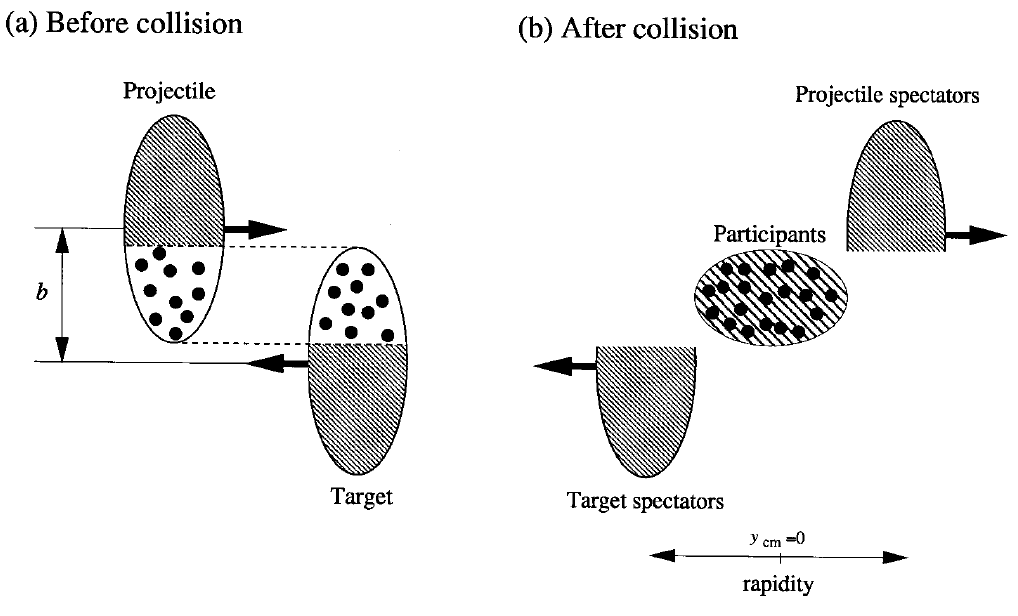
\includegraphics [width = 0.7\linewidth] {Intro/CollisionGeometry.png}
	\caption{Схематичное изображение Картина участника-зрителя о столкновении тяжелых ионов высокой энергии с прицельным параметром b. Слева (а) показаны два приближающихся ядра в центре масс. Справа (б) после столкновения нуклоны разделяются на участников, наблюдателей-снарядов и наблюдателей-мишеней.}
	\label{img:CollisionGeometry}  
\end{figure}


\subsection{Модель Глаубера}
Модель Глаубера [6] основана на простой геометрической картине ядерно-ядерного столкновения. Это полуклассическая модель, рассматривающая ядерные столкновения как множественные нуклон-нуклонные взаимодействия: нуклон налетающего ядра взаимодействует с нуклонами-мишенями с заданным распределением плотности. Предполагается, что нуклоны движутся по прямолинейным траекториям и не отклоняются даже после столкновений, что является допустимым приближением при энергиях $sqrt{s_{NN}} \sim 200$ ГэВ. Второе предположение состоит в том, что неупругое сечение нуклон-нуклонных взаимодействий $\sigma^{in}_{NN}$ не зависит от свойств среды и совпадает с $\sigma^{in}_{NN}$ в вакууме. Нуклоны распределены в ядре случайным образом в соответствии с распределением Вудса-Саксона. Плотность распределения нуклонов в ядре $\rho(r)$ определяется как
$$\rho(r) = \rho_0 \cdot \frac{1}{1+exp{\frac{r-R}{a}}}$$
где $R$ — радиус ядра, $а$ — параметр поверхностной диффузии. Профиль плотности золота показан на рис. \ref{img:WoodSaxon}. Для иона Au параметры $R$ = 6.38 фм, $a$ = 0.54 фм и $r_0$ = 0.169 фм$^{-3}$. Неупругое нуклон-нуклонное сечение $\sigma^{in}_{NN}$ = 42 мб используется для вычисления инвариантных спектров частиц в столкновениях тяжелых ионов.

\begin{figure}[] 
	\centerfloat
	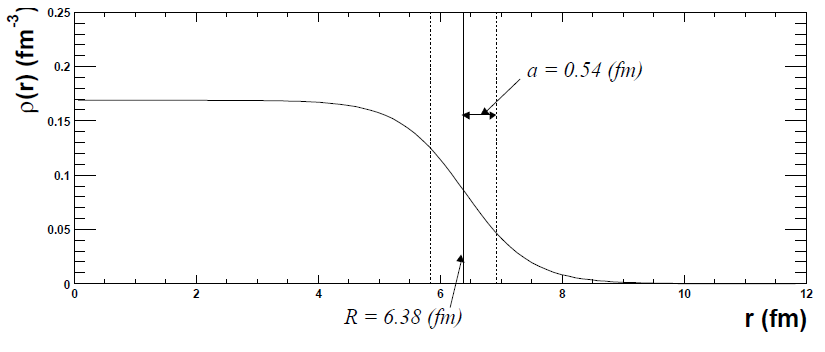
\includegraphics [width = 0.6\linewidth] {Intro/WoodSaxon.png}
	\caption{Профиль ядерной плотности Вудса-Саксона для Au.}
	\label{img:WoodSaxon}  
\end{figure}


\section{Отношения частиц и химическое равновесие}
Различия между механизмами рождения различных адронов могут быть установлены с помощью отношения их инвариантных спектров по поперечному импульсу. Установлено [], что отношения рожденных адронов хорошо описываются простой статистической моделью [].
\begin{figure}[ht] 
	\centerfloat
	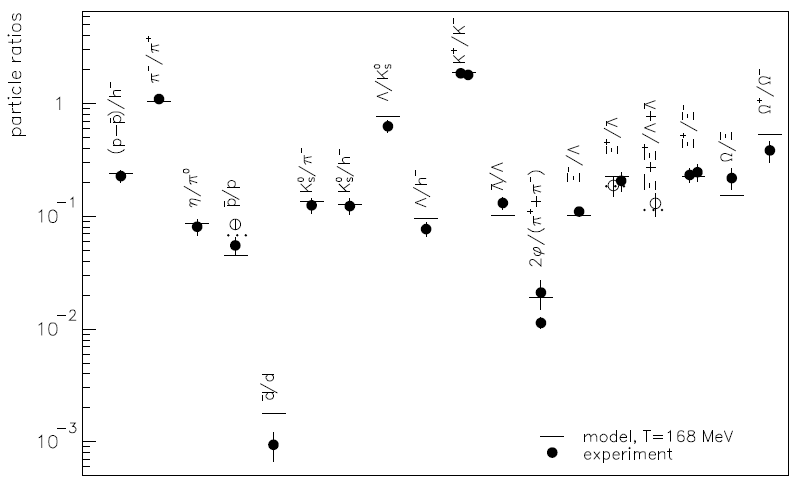
\includegraphics [width = 0.9\linewidth] {Intro/RatiosExp.png}
	\caption{Отношения выходов адронов. Сравнение между статистической моделью (горизонтальные линии) и экспериментальными отношениями (круги)} 
	\label{img:RatiosExp}  
\end{figure}

Статистическая модель основана на использовании большого канонического ансамбля для описания статистической суммы и, следовательно, плотности частиц вида $i$ в равновесном состоянии кварк-глонной материи:
\begin{equation}
	\label{eq:Ratio}
	n_i = \frac{g_i}{2 \pi ^2}\int_0^{\infty} \frac{p^2 dp}{exp[(E_i - \mu_i)/T_{ch}]\pm 1}
\end{equation}
где  $n_i$ - плотность частиц, $g_i$ - спиновое вырождение, $p$ - импульс, $E$ - полная энергия и $\mu_i =\mu_B B_i - \mu_S S_i - \mu_{I_3} I_{3i}$ - химический потенциал. Величины $B_i$, $S_i$ и $I_{3i}$ представляют собой барионное число, странность и третью компоненту изоспина для частицы вида $i$. В данной модели присутствуют только два параметра: температура $T_{ch}$ и барионный химический потенциал $\mu_B$, которые являются независимыми.  На рис. ??? показано сравнение измеренных интегральных отношений выходов частиц частиц и расчетов согласно статистической модели. Как видно из рисунка, данная модель хорошо согласовывается с экспериментальными данными.
Совпадаение экспериментальных данных с расчетсами статистической модели указывает на сохранение химического равновесия в системе. 

\subsection{Мотивация}

\begin{comment}

Систематическое изучение признаков формирования КГП в больших и малых системах столкновений позволит изучить свойства КГП..
Сошлёмся на библиографию.
Одна ссылка: \cite[с.~54]{Sokolov}\cite[с.~36]{Gaidaenko}.
Две ссылки: \cite{Sokolov,Gaidaenko}.
%Ссылка на собственные работы: \cite{vakbib1, confbib2}.
Много ссылок: %\cite[с.~54]{Lermontov,Management,Borozda} % такой «фокус»
%вызывает biblatex warning относительно опции sortcites, потому что неясно, к
%какому источнику относится уточнение о страницах, а bibtex об этой проблеме
%даже не предупреждает
\cite{Lermontov, Management, Borozda, Marketing, Constitution, FamilyCode,
    Gost.7.0.53, Razumovski, Lagkueva, Pokrovski, Methodology, Berestova,
    Kriger}%
\ifnumequal{\value{bibliosel}}{0}{% Примеры для bibtex8
    \cite{Sirotko, Lukina, Encyclopedia, Nasirova}%
}{% Примеры для biblatex через движок biber
    \cite{Sirotko2, Lukina2, Encyclopedia2, Nasirova2}%
}%
.
И~ещё немного ссылок:~\cite{Article,Book,Booklet,Conference,Inbook,Incollection,Manual,Mastersthesis,
    Misc,Phdthesis,Proceedings,Techreport,Unpublished}
% Следует обратить внимание, что пробел после запятой внутри \cite{}
% обрабатывается ожидаемо, а пробел перед запятой, может вызывать проблемы при
% обработке ссылок.
\cite{medvedev2006jelektronnye, CEAT:CEAT581, doi:10.1080/01932691.2010.513279,
    Gosele1999161,Li2007StressAnalysis, Shoji199895, test:eisner-sample,
    test:eisner-sample-shorted, AB_patent_Pomerantz_1968, iofis_patent1960}%
\ifnumequal{\value{bibliosel}}{0}{% Примеры для bibtex8
}{% Примеры для biblatex через движок biber
    \cite{patent2h, patent3h, patent2}%
}%
.

\ifnumequal{\value{bibliosel}}{0}{% Примеры для bibtex8
Попытка реализовать несколько ссылок на конкретные страницы
для \texttt{bibtex} реализации библиографии:
[\citenum{Sokolov}, с.~54; \citenum{Gaidaenko}, с.~36].
}{% Примеры для biblatex через движок biber
Несколько источников (мультицитата):
% Тут специально написано по-разному тире, для демонстрации, что
% применение специальных тире в настоящий момент в biblatex приводит к непоказу
% "с.".
\cites[vii--x, 5, 7]{Sokolov}[v"--~x, 25, 526]{Gaidaenko}[vii--x, 5, 7]{Techreport},
работает только в \texttt{biblatex} реализации библиографии.
}%

%Ссылки на собственные работы:~\cite{vakbib1, confbib1}.

Сошлёмся на приложения: Приложение~\cref{app:A}, Приложение~\cref{app:B2}.

Сошлёмся на формулу: формула~\cref{eq:equation1}.

Сошлёмся на изображение: рисунок~\cref{fig:knuth}.

Стандартной практикой является добавление к ссылкам префикса, характеризующего тип элемента.
Это не является строгим требованием, но~позволяет лучше ориентироваться в документах большого размера.
Например, для ссылок на~рисунки используется префикс \textit{fig},
для ссылки на~таблицу "--- \textit{tab}.

В таблице \cref{tab:tab_pref} приложения~\cref{app:B4} приведён список рекомендуемых
к использованию стандартных префиксов.

В некоторых ситуациях возникает необходимость отойти от требований ГОСТ по оформлению ссылок на
литературу.
В таком случае можно воспользоваться дополнительными опциями пакета \verb+biblatex+.

Например, в ссылке на книгу~\cite{sobenin_kdv} использование опции \verb+maxnames=4+ позволяет
вывести имена всех четырёх авторов.
По ГОСТ имена последних трёх авторов опускаются.

Кроме того, часто возникают проблемы с транслитерованными инициалами. Некоторые буквы русского
алфавита по правилам транслитерации записываются двумя буквами латинского алфавита (ю-yu, ё-yo и
т.д.).
Такие инициалы \verb+biblatex+ будет сокращать до одной буквы, что неверно.
Поправить его работу можно использовав опцию \verb+giveninits=false+.
Пример использования этой опции можно видеть в ссылке~\cite{initials}.

\section{Формулы}\label{sec:ch1/sec3}

Благодаря пакету \textit{icomma}, \LaTeX~одинаково хорошо воспринимает
в~качестве десятичного разделителя и запятую (\(3,1415\)), и точку (\(3.1415\)).

\subsection{Ненумерованные одиночные формулы}\label{subsec:ch1/sec3/sub1}

Вот так может выглядеть формула, которую необходимо вставить в~строку
по~тексту: \(x \approx \sin x\) при \(x \to 0\).

А вот так выглядит ненумерованная отдельностоящая формула c подстрочными
и надстрочными индексами:
\[
    (x_1+x_2)^2 = x_1^2 + 2 x_1 x_2 + x_2^2
\]

Формула с неопределенным интегралом:
\[
    \int f(\alpha+x)=\sum\beta
\]

При использовании дробей формулы могут получаться очень высокие:
\[
    \frac{1}{\sqrt{2}+
        \displaystyle\frac{1}{\sqrt{2}+
            \displaystyle\frac{1}{\sqrt{2}+\cdots}}}
\]

В формулах можно использовать греческие буквы:
%Все \original... команды заранее, ради этого примера, определены в Dissertation\userstyles.tex
\[
    \alpha\beta\gamma\delta\originalepsilon\epsilon\zeta\eta\theta%
    \vartheta\iota\kappa\varkappa\lambda\mu\nu\xi\pi\varpi\rho\varrho%
    \sigma\varsigma\tau\upsilon\originalphi\phi\chi\psi\omega\Gamma\Delta%
    \Theta\Lambda\Xi\Pi\Sigma\Upsilon\Phi\Psi\Omega
\]
\[%https://texfaq.org/FAQ-boldgreek
    \boldsymbol{\alpha\beta\gamma\delta\originalepsilon\epsilon\zeta\eta%
        \theta\vartheta\iota\kappa\varkappa\lambda\mu\nu\xi\pi\varpi\rho%
        \varrho\sigma\varsigma\tau\upsilon\originalphi\phi\chi\psi\omega\Gamma%
        \Delta\Theta\Lambda\Xi\Pi\Sigma\Upsilon\Phi\Psi\Omega}
\]

Для добавления формул можно использовать пары \verb+$+\dots\verb+$+ и \verb+$$+\dots\verb+$$+,
но~они считаются устаревшими.
Лучше использовать их функциональные аналоги \verb+\(+\dots\verb+\)+ и \verb+\[+\dots\verb+\]+.

\subsection{Ненумерованные многострочные формулы}\label{subsec:ch1/sec3/sub2}

Вот так можно написать две формулы, не нумеруя их, чтобы знаки <<равно>> были
строго друг под другом:
\begin{align}
    f_W & =  \min \left( 1, \max \left( 0, \frac{W_{soil} / W_{max}}{W_{crit}} \right)  \right), \nonumber \\
    f_T & =  \min \left( 1, \max \left( 0, \frac{T_s / T_{melt}}{T_{crit}} \right)  \right), \nonumber
\end{align}

Выровнять систему ещё и по переменной \( x \) можно, используя окружение
\verb|alignedat| из пакета \verb|amsmath|. Вот так:
\[
|x| = \left\{
\begin{alignedat}{2}
    &&x, \quad &\text{eсли } x\geqslant 0 \\
    &-&x, \quad & \text{eсли } x<0
\end{alignedat}
\right.
\]
Здесь первый амперсанд (в исходном \LaTeX\ описании формулы) означает
выравнивание по~левому краю, второй "--- по~\( x \), а~третий "--- по~слову
<<если>>. Команда \verb|\quad| делает большой горизонтальный пробел.

Ещё вариант:
\[
    |x|=
    \begin{cases}
        \phantom{-}x, \text{если } x \geqslant 0 \\
        -x, \text{если } x<0
    \end{cases}
\]

Кроме того, для  нумерованных формул \verb|alignedat| делает вертикальное
выравнивание номера формулы по центру формулы. Например, выравнивание
компонент вектора:
\begin{equation}
    \label{eq:2p3}
    \begin{alignedat}{2}
        {\mathbf{N}}_{o1n}^{(j)} = \,{\sin} \phi\,n\!\left(n+1\right)
        {\sin}\theta\,
        \pi_n\!\left({\cos} \theta\right)
        \frac{
        z_n^{(j)}\!\left( \rho \right)
        }{\rho}\,
        &{\boldsymbol{\hat{\mathrm e}}}_{r}\,+   \\
        +\,
        {\sin} \phi\,
        \tau_n\!\left({\cos} \theta\right)
        \frac{
        \left[\rho z_n^{(j)}\!\left( \rho \right)\right]^{\prime}
        }{\rho}\,
        &{\boldsymbol{\hat{\mathrm e}}}_{\theta}\,+   \\
        +\,
        {\cos} \phi\,
        \pi_n\!\left({\cos} \theta\right)
        \frac{
        \left[\rho z_n^{(j)}\!\left( \rho \right)\right]^{\prime}
        }{\rho}\,
        &{\boldsymbol{\hat{\mathrm e}}}_{\phi}\:.
    \end{alignedat}
\end{equation}

Ещё об отступах. Иногда для лучшей <<читаемости>> формул полезно
немного исправить стандартные интервалы \LaTeX\ с учётом логической
структуры самой формулы. Например в формуле~\cref{eq:2p3} добавлен
небольшой отступ \verb+\,+ между основными сомножителями, ниже
результат применения всех вариантов отступа:
\begin{align*}
    \backslash!             & \quad f(x) = x^2\! +3x\! +2         \\
    \mbox{по-умолчанию}     & \quad f(x) = x^2+3x+2               \\
    \backslash,             & \quad f(x) = x^2\, +3x\, +2         \\
    \backslash{:}           & \quad f(x) = x^2\: +3x\: +2         \\
    \backslash;             & \quad f(x) = x^2\; +3x\; +2         \\
    \backslash \mbox{space} & \quad f(x) = x^2\ +3x\ +2           \\
    \backslash \mbox{quad}  & \quad f(x) = x^2\quad +3x\quad +2   \\
    \backslash \mbox{qquad} & \quad f(x) = x^2\qquad +3x\qquad +2
\end{align*}

Можно использовать разные математические алфавиты:
\begin{align}
    \mathcal{ABCDEFGHIJKLMNOPQRSTUVWXYZ} \nonumber  \\
    \mathfrak{ABCDEFGHIJKLMNOPQRSTUVWXYZ} \nonumber \\
    \mathbb{ABCDEFGHIJKLMNOPQRSTUVWXYZ} \nonumber
\end{align}

Посмотрим на систему уравнений на примере аттрактора Лоренца:

\[
\left\{
\begin{array}{rl}
    \dot x = & \sigma (y-x)  \\
    \dot y = & x (r - z) - y \\
    \dot z = & xy - bz
\end{array}
\right.
\]

А для вёрстки матриц удобно использовать многоточия:
\[
    \left(
        \begin{array}{ccc}
            a_{11} & \ldots & a_{1n} \\
            \vdots & \ddots & \vdots \\
            a_{n1} & \ldots & a_{nn} \\
        \end{array}
    \right)
\]

\subsection{Нумерованные формулы}\label{subsec:ch1/sec3/sub3}

А вот так пишется нумерованная формула:
\begin{equation}
    \label{eq:equation1}
    e = \lim_{n \to \infty} \left( 1+\frac{1}{n} \right) ^n
\end{equation}

Нумерованных формул может быть несколько:
\begin{equation}
    \label{eq:equation2}
    \lim_{n \to \infty} \sum_{k=1}^n \frac{1}{k^2} = \frac{\pi^2}{6}
\end{equation}

Впоследствии на формулы~\cref{eq:equation1, eq:equation2} можно ссылаться.

Сделать так, чтобы номер формулы стоял напротив средней строки, можно,
используя окружение \verb|multlined| (пакет \verb|mathtools|) вместо
\verb|multline| внутри окружения \verb|equation|. Вот так:
\begin{equation} % \tag{S} % tag - вписывает свой текст
    \label{eq:equation3}
    \begin{multlined}
        1+ 2+3+4+5+6+7+\dots + \\
        + 50+51+52+53+54+55+56+57 + \dots + \\
        + 96+97+98+99+100=5050
    \end{multlined}
\end{equation}

Уравнения~\cref{eq:subeq_1,eq:subeq_2} демонстрируют возможности
окружения \verb|\subequations|.
\begin{subequations}
    \label{eq:subeq_1}
    \begin{gather}
        y = x^2 + 1 \label{eq:subeq_1-1} \\
        y = 2 x^2 - x + 1 \label{eq:subeq_1-2}
    \end{gather}
\end{subequations}
Ссылки на отдельные уравнения~\cref{eq:subeq_1-1,eq:subeq_1-2,eq:subeq_2-1}.
\begin{subequations}
    \label{eq:subeq_2}
    \begin{align}
        y & = x^3 + x^2 + x + 1 \label{eq:subeq_2-1} \\
        y & = x^2
    \end{align}
\end{subequations}

\subsection{Форматирование чисел и размерностей величин}\label{sec:units}

Числа форматируются при помощи команды \verb|\num|:
\num{5,3};
\num{2,3e8};
\num{12345,67890};
\num{2,6 d4};
\num{1+-2i};
\num{.3e45};
\num[exponent-base=2]{5 e64};
\num[exponent-base=2,exponent-to-prefix]{5 e64};
\num{1.654 x 2.34 x 3.430}
\num{1 2 x 3 / 4}.
Для написания последовательности чисел можно использовать команды \verb|\numlist| и \verb|\numrange|:
\numlist{10;30;50;70}; \numrange{10}{30}.
Значения углов можно форматировать при помощи команды \verb|\ang|:
\ang{2.67};
\ang{30,3};
\ang{-1;;};
\ang{;-2;};
\ang{;;-3};
\ang{300;10;1}.

Обратите внимание, что ГОСТ запрещает использование знака <<->> для обозначения отрицательных чисел
за исключением формул, таблиц и~рисунков.
Вместо него следует использовать слово <<минус>>.

Размерности можно записывать при помощи команд \verb|\si| и \verb|\SI|:
\si{\farad\squared\lumen\candela};
\si{\joule\per\mole\per\kelvin};
\si[per-mode = symbol-or-fraction]{\joule\per\mole\per\kelvin};
\si{\metre\per\second\squared};
\SI{0.10(5)}{\neper};
\SI{1.2-3i e5}{\joule\per\mole\per\kelvin};
\SIlist{1;2;3;4}{\tesla};
\SIrange{50}{100}{\volt}.
Список единиц измерений приведён в таблицах~\cref{tab:unit:base,
    tab:unit:derived,tab:unit:accepted,tab:unit:physical,tab:unit:other}.
Приставки единиц приведены в~таблице~\cref{tab:unit:prefix}.

С дополнительными опциями форматирования можно ознакомиться в~описании пакета \texttt{siunitx};
изменить или добавить единицы измерений можно в~файле \texttt{siunitx.cfg}.

\begin{table}
    \centering
    \captionsetup{justification=centering} % выравнивание подписи по-центру
    \caption{Основные величины СИ}\label{tab:unit:base}
    \begin{tabular}{llc}
        \toprule
        Название  & Команда                 & Символ         \\
        \midrule
        Ампер     & \verb|\ampere| & \si{\ampere}   \\
        Кандела   & \verb|\candela| & \si{\candela}  \\
        Кельвин   & \verb|\kelvin| & \si{\kelvin}   \\
        Килограмм & \verb|\kilogram| & \si{\kilogram} \\
        Метр      & \verb|\metre| & \si{\metre}    \\
        Моль      & \verb|\mole| & \si{\mole}     \\
        Секунда   & \verb|\second| & \si{\second}   \\
        \bottomrule
    \end{tabular}
\end{table}

\begin{table}
    \small
    \centering
    \begin{threeparttable}% выравнивание подписи по границам таблицы
        \caption{Производные единицы СИ}\label{tab:unit:derived}
        \begin{tabular}{llc|llc}
            \toprule
            Название       & Команда                 & Символ              & Название & Команда & Символ \\
            \midrule
            Беккерель      & \verb|\becquerel| & \si{\becquerel}     &
            Ньютон         & \verb|\newton| & \si{\newton}                                      \\
            Градус Цельсия & \verb|\degreeCelsius| & \si{\degreeCelsius} &
            Ом             & \verb|\ohm| & \si{\ohm}                                         \\
            Кулон          & \verb|\coulomb| & \si{\coulomb}       &
            Паскаль        & \verb|\pascal| & \si{\pascal}                                      \\
            Фарад          & \verb|\farad| & \si{\farad}         &
            Радиан         & \verb|\radian| & \si{\radian}                                      \\
            Грей           & \verb|\gray| & \si{\gray}          &
            Сименс         & \verb|\siemens| & \si{\siemens}                                     \\
            Герц           & \verb|\hertz| & \si{\hertz}         &
            Зиверт         & \verb|\sievert| & \si{\sievert}                                     \\
            Генри          & \verb|\henry| & \si{\henry}         &
            Стерадиан      & \verb|\steradian| & \si{\steradian}                                   \\
            Джоуль         & \verb|\joule| & \si{\joule}         &
            Тесла          & \verb|\tesla| & \si{\tesla}                                       \\
            Катал          & \verb|\katal| & \si{\katal}         &
            Вольт          & \verb|\volt| & \si{\volt}                                        \\
            Люмен          & \verb|\lumen| & \si{\lumen}         &
            Ватт           & \verb|\watt| & \si{\watt}                                        \\
            Люкс           & \verb|\lux| & \si{\lux}           &
            Вебер          & \verb|\weber| & \si{\weber}                                       \\
            \bottomrule
        \end{tabular}
    \end{threeparttable}
\end{table}

\begin{table}
    \centering
    \begin{threeparttable}% выравнивание подписи по границам таблицы
        \caption{Внесистемные единицы}\label{tab:unit:accepted}

        \begin{tabular}{llc}
            \toprule
            Название        & Команда                 & Символ          \\
            \midrule
            День            & \verb|\day| & \si{\day}       \\
            Градус          & \verb|\degree| & \si{\degree}    \\
            Гектар          & \verb|\hectare| & \si{\hectare}   \\
            Час             & \verb|\hour| & \si{\hour}      \\
            Литр            & \verb|\litre| & \si{\litre}     \\
            Угловая минута  & \verb|\arcminute| & \si{\arcminute} \\
            Угловая секунда & \verb|\arcsecond| & \si{\arcsecond} \\ %
            Минута          & \verb|\minute| & \si{\minute}    \\
            Тонна           & \verb|\tonne| & \si{\tonne}     \\
            \bottomrule
        \end{tabular}
    \end{threeparttable}
\end{table}

\begin{table}
    \centering
    \captionsetup{justification=centering}
    \caption{Внесистемные единицы, получаемые из эксперимента}\label{tab:unit:physical}
    \begin{tabular}{llc}
        \toprule
        Название                & Команда                 & Символ                 \\
        \midrule
        Астрономическая единица & \verb|\astronomicalunit| & \si{\astronomicalunit} \\
        Атомная единица массы   & \verb|\atomicmassunit| & \si{\atomicmassunit}   \\
        Боровский радиус        & \verb|\bohr| & \si{\bohr}             \\
        Скорость света          & \verb|\clight| & \si{\clight}           \\
        Дальтон                 & \verb|\dalton| & \si{\dalton}           \\
        Масса электрона         & \verb|\electronmass| & \si{\electronmass}     \\
        Электрон Вольт          & \verb|\electronvolt| & \si{\electronvolt}     \\
        Элементарный заряд      & \verb|\elementarycharge| & \si{\elementarycharge} \\
        Энергия Хартри          & \verb|\hartree| & \si{\hartree}          \\
        Постоянная Планка       & \verb|\planckbar| & \si{\planckbar}        \\
        \bottomrule
    \end{tabular}
\end{table}

\begin{table}
    \centering
    \begin{threeparttable}% выравнивание подписи по границам таблицы
        \caption{Другие внесистемные единицы}\label{tab:unit:other}
        \begin{tabular}{llc}
            \toprule
            Название                  & Команда                 & Символ             \\
            \midrule
            Ангстрем                  & \verb|\angstrom| & \si{\angstrom}     \\
            Бар                       & \verb|\bar| & \si{\bar}          \\
            Барн                      & \verb|\barn| & \si{\barn}         \\
            Бел                       & \verb|\bel| & \si{\bel}          \\
            Децибел                   & \verb|\decibel| & \si{\decibel}      \\
            Узел                      & \verb|\knot| & \si{\knot}         \\
            Миллиметр ртутного столба & \verb|\mmHg| & \si{\mmHg}         \\
            Морская миля              & \verb|\nauticalmile| & \si{\nauticalmile} \\
            Непер                     & \verb|\neper| & \si{\neper}        \\
            \bottomrule
        \end{tabular}
    \end{threeparttable}
\end{table}

\begin{table}
    \small
    \centering
    \begin{threeparttable}% выравнивание подписи по границам таблицы
        \caption{Приставки СИ}\label{tab:unit:prefix}
        \begin{tabular}{llcc|llcc}
            \toprule
            Приставка & Команда                  & Символ      & Степень &
            Приставка & Команда                  & Символ      & Степень   \\
            \midrule
            Иокто     & \verb|\yocto|  & \si{\yocto} & -24     &
            Дека      & \verb|\deca|  & \si{\deca}  & 1         \\
            Зепто     & \verb|\zepto|  & \si{\zepto} & -21     &
            Гекто     & \verb|\hecto|  & \si{\hecto} & 2         \\
            Атто      & \verb|\atto|  & \si{\atto}  & -18     &
            Кило      & \verb|\kilo|  & \si{\kilo}  & 3         \\
            Фемто     & \verb|\femto|  & \si{\femto} & -15     &
            Мега      & \verb|\mega|  & \si{\mega}  & 6         \\
            Пико      & \verb|\pico|  & \si{\pico}  & -12     &
            Гига      & \verb|\giga|  & \si{\giga}  & 9         \\
            Нано      & \verb|\nano|  & \si{\nano}  & -9      &
            Терра     & \verb|\tera|  & \si{\tera}  & 12        \\
            Микро     & \verb|\micro|  & \si{\micro} & -6      &
            Пета      & \verb|\peta|  & \si{\peta}  & 15        \\
            Милли     & \verb|\milli|  & \si{\milli} & -3      &
            Екса      & \verb|\exa|  & \si{\exa}   & 18        \\
            Санти     & \verb|\centi|  & \si{\centi} & -2      &
            Зетта     & \verb|\zetta|  & \si{\zetta} & 21        \\
            Деци      & \verb|\deci| & \si{\deci}  & -1      &
            Иотта     & \verb|\yotta| & \si{\yotta} & 24        \\
            \bottomrule
        \end{tabular}
    \end{threeparttable}
\end{table}

\subsection{Заголовки с формулами: \texorpdfstring{\(a^2 + b^2 = c^2\)}{%
        a\texttwosuperior\ + b\texttwosuperior\ = c\texttwosuperior},
    \texorpdfstring{\(\left\vert\textrm{{Im}}\Sigma\left(
            \protect\varepsilon\right)\right\vert\approx const\)}{|ImΣ (ε)| ≈ const},
    \texorpdfstring{\(\sigma_{xx}^{(1)}\)}{σ\_\{xx\}\textasciicircum\{(1)\}}
}\label{subsec:with_math}

Пакет \texttt{hyperref} берёт текст для закладок в pdf-файле из~аргументов
команд типа \verb|\section|, которые могут содержать математические формулы,
а~также изменения цвета текста или шрифта, которые не отображаются в~закладках.
Чтобы использование формул в заголовках не вызывало в~логе компиляции появление
предупреждений типа <<\texttt{Token not allowed in~a~PDF string
    (Unicode):(hyperref) removing...}>>, следует использовать конструкцию
\verb|\texorpdfstring{}{}|, где в~первых фигурных скобках указывается
формула, а~во~вторых "--- запись формулы для закладок.

\section{Рецензирование текста}\label{sec:markup}

В шаблоне для диссертации и автореферата заданы команды рецензирования.
Они видны при компиляции шаблона в режиме черновика или при установке
соответствующей настройки (\verb+showmarkup+) в~файле \verb+common/setup.tex+.

Команда \verb+\todo+ отмечает текст красным цветом.
\todo{Например, так.}

Команда \verb+\note+ позволяет выбрать цвет текста.
\note{Чёрный, } \note[red]{красный, } \note[green]{зелёный, }
\note[blue]{синий.} \note[orange]{Обратите внимание на ширину и расстановку
    формирующихся пробелов, в~результате приведённой записи (зависит также
    от~применяемого компилятора).}

Окружение \verb+commentbox+ также позволяет выбрать цвет.

\begin{commentbox}[red]
    Красный текст.

    Несколько параграфов красного текста.
\end{commentbox}

\begin{commentbox}[blue]
    Синяя формула.

    \begin{equation}
        \alpha + \beta = \gamma
    \end{equation}
\end{commentbox}

\verb+commentbox+ позволяет закомментировать участок кода в~режиме чистовика.
Чтобы убрать кусок кода для всех режимов, можно использовать окружение
\verb+comment+.


\section{Работа со списком сокращений и~условных обозначений}\label{sec:acronyms}

С помощью пакета \texttt{nomencl} можно создавать удобный сортированный список
сокращений и условных обозначений во время написания текста. Вызов
\verb+\nomenclature+ добавляет нужный символ или сокращение с~описанием
в~список, который затем печатается вызовом \verb+\printnomenclature+
в~соответствующем разделе.
Для того, чтобы эти операции прошли, потребуется дополнительный вызов
\verb+makeindex -s nomencl.ist -o %.nls %.nlo+ в~командной строке, где вместо
\verb+%+ следует подставить имя главного файла проекта (\verb+dissertation+
для этого шаблона).
Затем потребуется один или два дополнительных вызова компилятора проекта.
\begin{equation}
    \omega = c k,
\end{equation}
где \( \omega \) "--- частота света, \( c \) "--- скорость света, \( k \) "---
модуль волнового вектора.
\nomenclature{\(\omega\)}{частота света\nomrefeq}
\nomenclature{\(c\)}{скорость света\nomrefpage}
\nomenclature{\(k\)}{модуль волнового вектора\nomrefeqpage}
Использование
\begin{verbatim}
\nomenclature{\(\omega\)}{частота света\nomrefeq}
\nomenclature{\(c\)}{скорость света\nomrefpage}
\nomenclature{\(k\)}{модуль волнового вектора\nomrefeqpage}
\end{verbatim}
после уравнения добавит в список условных обозначений три записи.
Ссылки \verb+\nomrefeq+ на последнее уравнение, \verb+\nomrefpage+ "--- на
страницу, \verb+\nomrefeqpage+ "--- сразу на~последнее уравнение и~на~страницу,
можно опускать и~не~использовать.

Группировкой и сортировкой пунктов в списке можно управлять с~помощью указания
дополнительных аргументов к команде \verb+nomenclature+.
Например, при вызове
\begin{verbatim}
\nomenclature[03]{\( \hbar \)}{постоянная Планка}
\nomenclature[01]{\( G \)}{гравитационная постоянная}
\end{verbatim}
\( G \) будет стоять в списке выше, чем \( \hbar \).
Для корректных вертикальных отступов между строками в описании лучше
не~использовать многострочные формулы в~списке обозначений.

\nomenclature{%
    \( \begin{rcases}
        a_n \\
        b_n
    \end{rcases} \)%
}{коэффициенты разложения Ми в дальнем поле соответствующие электрическим и
    магнитным мультиполям}
\nomenclature[a\( e \)]{\( {\boldsymbol{\hat{\mathrm e}}} \)}{единичный вектор}
\nomenclature{\( E_0 \)}{амплитуда падающего поля}
\nomenclature{\( j \)}{тип функции Бесселя}
\nomenclature{\( k \)}{волновой вектор падающей волны}
\nomenclature{%
    \( \begin{rcases}
        a_n \\
        b_n
    \end{rcases} \)%
}{и снова коэффициенты разложения Ми в дальнем поле соответствующие
    электрическим и магнитным мультиполям. Добавлено много текста, так что
    описание группы условных обозначений значительно превысило высоту этой
    группы...}
\nomenclature{\( L \)}{общее число слоёв}
\nomenclature{\( l \)}{номер слоя внутри стратифицированной сферы}
\nomenclature{\( \lambda \)}{длина волны электромагнитного излучения в вакууме}
\nomenclature{\( n \)}{порядок мультиполя}
\nomenclature{%
    \( \begin{rcases}
        {\mathbf{N}}_{e1n}^{(j)} & {\mathbf{N}}_{o1n}^{(j)} \\
        {\mathbf{M}_{o1n}^{(j)}} & {\mathbf{M}_{e1n}^{(j)}}
    \end{rcases} \)%
}{сферические векторные гармоники}
\nomenclature{\( \mu \)}{магнитная проницаемость в вакууме}
\nomenclature{\( r, \theta, \phi \)}{полярные координаты}
\nomenclature{\( \omega \)}{частота падающей волны}

С помощью \verb+nomenclature+ можно включать в~список сокращения,
не~используя их~в~тексте.
% запись сокращения в список происходит командой \nomenclature,
% а не употреблением самого сокращения
\nomenclature{FEM}{finite element method, метод конечных элементов}
\nomenclature{FIT}{finite integration technique, метод конечных интегралов}
\nomenclature{FMM}{fast multipole method, быстрый метод многополюсника}
\nomenclature{FVTD}{finite volume time-domain, метод конечных объёмов
    во~временной области}
\nomenclature{MLFMA}{multilevel fast multipole algorithm, многоуровневый
    быстрый алгоритм многополюсника}
\nomenclature{BEM}{boundary element method, метод граничных элементов}
\nomenclature{CST MWS}{Computer Simulation Technology Microwave Studio
    программа для компьютерного моделирования уравнен Максвелла}
\nomenclature{DDA}{discrete dipole approximation, приближение дискретиных
    диполей}
\nomenclature{FDFD}{finite difference frequency domain, метод конечных
    разностей в~частотной области}
\nomenclature{FDTD}{finite difference time domain, метод конечных разностей
    во~временной области}
\nomenclature{MoM}{method of moments, метод моментов}
\nomenclature{MSTM}{multiple sphere T-Matrix, метод Т-матриц для множества
    сфер}
\nomenclature{PSTD}{pseudospectral time domain method, псевдоспектральный метод
    во~временной области}
\nomenclature{TLM}{transmission line matrix method, метод матриц линий передач}

\FloatBarrier
\end{comment}
